% 若编译失败,且生成 .synctex(busy) 辅助文件,可能有两个原因:
% 1. 需要插入的图片不存在:Ctrl + F 搜索 'figure' 将这些代码注释/删除掉即可
% 2. 路径/文件名含中文或空格:更改路径/文件名即可

% --------------------- 文章宏包及相关设置 --------------------- %
% >> ------------------ 文章宏包及相关设置 ------------------ << %
% 设定文章类型与编码格式
\documentclass[UTF8]{article}		

% 物理实验报告所需的其它宏包
\usepackage{ulem}   % \uline 下划线支持
\usepackage{circuitikz} % 电路图 tikz 支持
\usepackage{pdfpages}   % 用于导入 pdf 文件

% 本 .tex 专属的宏定义
    \def\V{\ \mathrm{V}}
    \def\uV{\ \mu\mathrm{V}}
    \def\mV{\ \mathrm{mV}}
    \def\K{\ \mathrm{K}}
    \def\kV{\ \mathrm{KV}}
    \def\KV{\ \mathrm{KV}}
    \def\MV{\ \mathrm{MV}}
    \def\uA{\ \mu\mathrm{A}}
    \def\mA{\ \mathrm{mA}}
    \def\A{\ \mathrm{A}}
    \def\kA{\ \mathrm{KA}}
    \def\KA{\ \mathrm{KA}}
    \def\MA{\ \mathrm{MA}}
    \def\O{\ \Omega}
    \def\mO{\ \Omega}
    \def\kO{\ \mathrm{K}\Omega}
    \def\KO{\ \mathrm{K}\Omega}
    \def\MO{\ \mathrm{M}\Omega}
    \def\Hz{\ \mathrm{Hz}}
    \def\uF{\ \mu\mathrm{F}}
    \def\mF{\ \mathrm{mF}}
    \def\F{\ \mathrm{F}}
    \def\Re{\mathrm{\,Re}\,}
    \def\Im{\mathrm{\,Im}\,}
    \def\sinc{\mathrm{\,sinc}\,}

% 自定义宏定义
    \def\N{\mathbb{N}}
    \def\F{\mathbb{F}}
    \def\Z{\mathbb{Z}}
    \def\Q{\mathbb{Q}}
    \def\R{\mathbb{R}}
    \def\C{\mathbb{C}}
    \def\T{\mathbb{T}}
    \def\S{\mathbb{S}}
    %\def\A{\mathbb{A}}
    \def\I{\mathscr{I}}
    \def\d{\mathrm{d}}
    \def\p{\partial}


% 导入基本宏包
    \usepackage[UTF8]{ctex}     % 设置文档为中文语言
    \usepackage{hyperref}  % 宏包:自动生成超链接 (此宏包与标题中的数学环境冲突)
    \hypersetup{
        colorlinks=true,    % false:边框链接 ; true:彩色链接
        citecolor={blue},    % 文献引用颜色
        linkcolor={blue},   % 目录 (我们在目录处单独设置),公式,图表,脚注等内部链接颜色
        urlcolor={orange},    % 网页 URL 链接颜色,包括 \href 中的 text
        % cyan 浅蓝色 
        % magenta 洋红色
        % yellow 黄色
        % black 黑色
        % white 白色
        % red 红色
        % green 绿色
        % blue 蓝色
        % gray 灰色
        % darkgray 深灰色
        % lightgray 浅灰色
        % brown 棕色
        % lime 石灰色
        % olive 橄榄色
        % orange 橙色
        % pink 粉红色
        % purple 紫色
        % teal 蓝绿色
        % violet 紫罗兰色
    }
    % \usepackage{docmute}    % 宏包:子文件导入时自动去除导言区,用于主/子文件的写作方式,\include{./51单片机笔记}即可。注:启用此宏包会导致.tex文件capacity受限。
    \usepackage{amsmath}    % 宏包:数学公式
    \usepackage{mathrsfs}   % 宏包:提供更多数学符号
    \usepackage{amssymb}    % 宏包:提供更多数学符号
    \usepackage{pifont}     % 宏包:提供了特殊符号和字体
    \usepackage{extarrows}  % 宏包:更多箭头符号 
    \usepackage{multicol}   % 宏包:支持多栏 

% 文章页面margin设置
    \usepackage[a4paper]{geometry}
        \geometry{top=0.75in}
        \geometry{bottom=0.75in}
        \geometry{left=0.75in}
        \geometry{right=0.75in}   % 设置上下左右页边距
        \geometry{marginparwidth=1.75cm}    % 设置边注距离(注释、标记等)

% 配置数学环境
    \usepackage{amsthm} % 宏包:数学环境配置
    % theorem-line 环境自定义
        \newtheoremstyle{MyLineTheoremStyle}% <name>
            {11pt}% <space above>
            {11pt}% <space below>
            {\kaishu}% <body font> 默认使用正文字体, \kaishu 为楷体
            {}% <indent amount>
            {\bfseries}% <theorem head font> 设置标题项为加粗
            {:\ \ }% <punctuation after theorem head>
            {.5em}% <space after theorem head>
            {\textbf{#1}\thmnumber{#2}\ \ (\,\textbf{#3}\,)}% 设置标题内容顺序
        \theoremstyle{MyLineTheoremStyle} % 应用自定义的定理样式
        \newtheorem{LineTheorem}{Theorem.\,}
    % theorem-block 环境自定义
        \newtheoremstyle{MyBlockTheoremStyle}% <name>
            {11pt}% <space above>
            {11pt}% <space below>
            {\kaishu}% <body font> 使用默认正文字体
            {}% <indent amount>
            {\bfseries}% <theorem head font> 设置标题项为加粗
            {:\\ \indent}% <punctuation after theorem head>
            {.5em}% <space after theorem head>
            {\textbf{#1}\thmnumber{#2}\ \ (\,\textbf{#3}\,)}% 设置标题内容顺序
        \theoremstyle{MyBlockTheoremStyle} % 应用自定义的定理样式
        \newtheorem{BlockTheorem}[LineTheorem]{Theorem.\,} % 使用 LineTheorem 的计数器
    % definition 环境自定义
        \newtheoremstyle{MySubsubsectionStyle}% <name>
            {11pt}% <space above>
            {11pt}% <space below>
            {}% <body font> 使用默认正文字体
            {}% <indent amount>
            {\bfseries}% <theorem head font> 设置标题项为加粗
            {:\\ \indent}% <punctuation after theorem head>
            {0pt}% <space after theorem head>
            {\textbf{#3}}% 设置标题内容顺序
        \theoremstyle{MySubsubsectionStyle} % 应用自定义的定理样式
        \newtheorem{definition}{}

%宏包:有色文本框(proof环境)及其设置
    \usepackage{xcolor}    %设置插入的文本框颜色
    \usepackage[strict]{changepage}     % 提供一个 adjustwidth 环境
    \usepackage{framed}     % 实现方框效果
        \definecolor{graybox_color}{rgb}{0.95,0.95,0.96} % 文本框颜色。修改此行中的 rgb 数值即可改变方框纹颜色,具体颜色的rgb数值可以在网站https://colordrop.io/ 中获得。(截止目前的尝试还没有成功过,感觉单位不一样)(找到喜欢的颜色,点击下方的小眼睛,找到rgb值,复制修改即可)
        \newenvironment{graybox}{%
        \def\FrameCommand{%
        \hspace{1pt}%
        {\color{gray}\vrule width 2pt}%
        {\color{graybox_color}\vrule width 4pt}%
        \colorbox{graybox_color}%
        }%
        \MakeFramed{\advance\hsize-\width\FrameRestore}%
        \noindent\hspace{-4.55pt}% disable indenting first paragraph
        \begin{adjustwidth}{}{7pt}%
        \vspace{2pt}\vspace{2pt}%
        }
        {%
        \vspace{2pt}\end{adjustwidth}\endMakeFramed%
        }

% 外源代码插入设置
    % matlab 代码插入设置
    \usepackage{matlab-prettifier}
        \lstset{style=Matlab-editor}    % 继承 matlab 代码高亮 , 此行不能删去
    \usepackage[most]{tcolorbox} % 引入tcolorbox包 
    \usepackage{listings} % 引入listings包
        \tcbuselibrary{listings, skins, breakable}
        \newfontfamily\codefont{Consolas} % 定义需要的 codefont 字体
        \lstdefinestyle{MatlabStyle_inc}{   % 插入代码的样式
            language=Matlab,
            basicstyle=\footnotesize\ttfamily\codefont,    % ttfamily 确保等宽 
            breakatwhitespace=false,
            breaklines=true,
            captionpos=b,
            keepspaces=true,
            numbers=left,
            numbersep=15pt,
            showspaces=false,
            showstringspaces=false,
            showtabs=false,
            tabsize=2,
            xleftmargin=15pt,   % 左边距
            %frame=single, % single 为包围式单线框
            frame=shadowbox,    % shadowbox 为带阴影包围式单线框效果
            %escapeinside=``,   % 允许在代码块中使用 LaTeX 命令 (此行无用)
            %frameround=tttt,    % tttt 表示四个角都是圆角
            framextopmargin=0pt,    % 边框上边距
            framexbottommargin=0pt, % 边框下边距
            framexleftmargin=5pt,   % 边框左边距
            framexrightmargin=5pt,  % 边框右边距
            rulesepcolor=\color{red!20!green!20!blue!20}, % 阴影框颜色设置
            %backgroundcolor=\color{blue!10}, % 背景颜色
        }
        \lstdefinestyle{MatlabStyle_src}{   % 插入代码的样式
            language=Matlab,
            basicstyle=\small\ttfamily\codefont,    % ttfamily 确保等宽 
            breakatwhitespace=false,
            breaklines=true,
            captionpos=b,
            keepspaces=true,
            numbers=left,
            numbersep=15pt,
            showspaces=false,
            showstringspaces=false,
            showtabs=false,
            tabsize=2,
        }
        \newtcblisting{matlablisting}{
            %arc=2pt,        % 圆角半径
            % 调整代码在 listing 中的位置以和引入文件时的格式相同
            top=0pt,
            bottom=0pt,
            left=-5pt,
            right=-5pt,
            listing only,   % 此句不能删去
            listing style=MatlabStyle_src,
            breakable,
            colback=white,   % 选一个合适的颜色
            colframe=black!0,   % 感叹号后跟不透明度 (为 0 时完全透明)
        }
        \lstset{
            style=MatlabStyle_inc,
        }

% table 支持
    \usepackage{booktabs}   % 宏包:三线表
    \usepackage{tabularray} % 宏包:表格排版
    \usepackage{longtable}  % 宏包:长表格

% figure 设置
    \usepackage{graphicx}  % 支持 jpg, png, eps, pdf 图片 
    \usepackage{svg}       % 支持 svg 图片
        \svgsetup{
            % 指向 inkscape.exe 的路径
            inkscapeexe = C:/aa_MySame/inkscape/bin/inkscape.exe, 
            % 一定程度上修复导入后图片文字溢出几何图形的问题
            inkscapelatex = false                 
        }
    \usepackage{subcaption} % 用于子图和小图注  

% 图表进阶设置
    \usepackage{caption}    % 图注、表注
        \captionsetup[figure]{name=图}  
        \captionsetup[table]{name=表}
        \captionsetup{
            labelfont=bf, % 设置标签为粗体
            textfont=bf,  % 设置文本为粗体
            font=small  
        }
    \usepackage{float}     % 图表位置浮动设置 
    \usepackage{etoolbox} % 用于保证图注表注的数学字符为粗体
        \AtBeginEnvironment{figure}{\boldmath} % 图注中的数学字符为粗体
        \AtBeginEnvironment{table}{\boldmath}  % 表注中的数学字符为粗体
        \AtBeginEnvironment{tabular}{\unboldmath}   % 保证表格中的数学字符不受额外影响

% 圆圈序号自定义
    \newcommand*\circled[1]{\tikz[baseline=(char.base)]{\node[shape=circle,draw,inner sep=0.8pt, line width = 0.03em] (char) {\bfseries #1};}}   % TikZ solution

% 列表设置
    \usepackage{enumitem}   % 宏包:列表环境设置
        \setlist[enumerate]{
            label=(\arabic*) ,   % 设置序号样式为加粗的 (1) (2) (3)
            ref=\arabic*, % 如果需要引用列表项,这将决定引用格式(这里仍然使用数字)
            itemsep=0pt, parsep=0pt, topsep=0pt, partopsep=0pt, leftmargin=3.5em} 
        \setlist[itemize]{itemsep=0pt, parsep=0pt, topsep=0pt, partopsep=0pt, leftmargin=3.5em}
        \newlist{circledenum}{enumerate}{1} % 创建一个新的枚举环境  
        \setlist[circledenum,1]{  
            label=\protect\circled{\arabic*}, % 使用 \arabic* 来获取当前枚举计数器的值,并用 \circled 包装它  
            ref=\arabic*, % 如果需要引用列表项,这将决定引用格式(这里仍然使用数字)
            itemsep=0pt, parsep=0pt, topsep=0pt, partopsep=0pt, leftmargin=3.5em
        }  

% 其它设置
    % 脚注设置
        \renewcommand\thefootnote{\ding{\numexpr171+\value{footnote}}}
    % 参考文献引用设置
        \bibliographystyle{unsrt}   % 设置参考文献引用格式为unsrt
        \newcommand{\upcite}[1]{\textsuperscript{\cite{#1}}}     % 自定义上角标式引用
    % 文章序言设置
        \newcommand{\cnabstractname}{序言}
        \newenvironment{cnabstract}{%
            \par\Large
            \noindent\mbox{}\hfill{\bfseries \cnabstractname}\hfill\mbox{}\par
            \vskip 2.5ex
            }{\par\vskip 2.5ex}

% 文章默认字体设置
    \usepackage{fontspec}   % 宏包:字体设置
        \setmainfont{SimSun}    % 设置中文字体为宋体字体
        \setCJKmainfont[AutoFakeBold=3]{SimSun} % 设置加粗字体为 SimSun 族,AutoFakeBold 可以调整字体粗细
        \setmainfont{Times New Roman} % 设置英文字体为Times New Roman

% 各级标题自定义设置
    \usepackage{titlesec}   
        % section标题自定义设置 
        \titleformat{\section}[hang]{\normalfont\Large\bfseries\boldmath}{\thesection}{8pt}{}
        % subsection 标题自定义设置
        \titleformat{\subsection}[hang]{\normalfont\large\bfseries\boldmath}{\thesubsection}{8pt}{}
        \titlespacing*{\subsection}{0pt}{10pt}{6pt} % 控制上下间距


% --------------------- 文章宏包及相关设置 --------------------- %
% >> ------------------ 文章宏包及相关设置 ------------------ << %


% ------------------------ 文章信息区 ------------------------ %
% ------------------------ 文章信息区 ------------------------ %
% 页眉页脚设置
\usepackage{fancyhdr}   %宏包:页眉页脚设置
    \pagestyle{fancy}
    \fancyhf{}
    \cfoot{\thepage}
    \renewcommand\headrulewidth{1pt}
    \renewcommand\footrulewidth{0pt}
    \rhead{\bfseries \large {\color{red} 分组序号: 2-05}}    
    \chead{《基础物理实验》实验报告,\ 丁毅,\ 2023K8009908031}
    \lhead{\small Ex.10 傅里叶光学 (2024.11.05)}

% 开始编辑文章

\begin{document}
\begin{center}\large
    \vspace*{-0.8cm}
    \noindent{\huge\bfseries《\ \ 基\ \ 础\ \ 物\ \ 理\ \ 实\ \ 验\ \ \ 》\ \ 实\ \ 验\ \ 报\ \ 告 }
    \\\vspace{0.1cm}
    \noindent{
    {\bfseries 
    实验名称:\uline{\hspace{1.9cm} 傅里叶光学基础 \hspace{1.9cm}}
    }\hspace{0.4cm}
    指导教师:\uline{\hspace{0.3cm}张秋琳 \ \ qlzhang@iphy.ac.cn\hspace{0.3cm}}
    }
    \\\vspace{0.1cm}
    \noindent
    {
    姓名:\uline{\,\,\,丁毅\,\,\,}\hspace{0.2cm}
    学号:\uline{\,\,\,{ 2023K8009908031}\,\,\,}\hspace{0.2cm}
    班级/专业:\uline{\,\,\,{2308/电子信息}\,\,\,}\hspace{0.2cm}
    分组序号:\uline{\,\,\,{2-05}\,\,\,}
    }
    \\\vspace{0.1cm}
    \noindent{
    实验日期:\uline{\,\,{ 2024.11.05}\,\,}\hspace{0.2cm}
    实验地点:\uline{\,\,\,教学楼{ 705}\,\,\,}\hspace{0.2cm}
    是否调课/补课:\uline{\hspace{0.26cm}否 \hspace{0.26cm}}\hspace{0.2cm}
    成绩:\uline{\hspace{2cm}}
    }
\end{center}
\vspace{-0.4cm}
\noindent\rule{\textwidth}{0.075em}   % 分割线
\vspace{-1.0cm}
% ------------------------ 文章信息区 ------------------------ %
% ------------------------ 文章信息区 ------------------------ %


% 目录
\setcounter{tocdepth}{2}  % 目录深度为 2(不显示 subsubsection)
\noindent\tableofcontents\thispagestyle{fancy}   % 显示页码、页眉等

\newpage
\rhead{\bfseries\small 分组序号: 2-05}

\begin{graybox}
考虑到本次实验的特殊性,在每一子实验下分别列写实验目的、原理及步骤,并紧跟实验结论与分析,而不统一将原理写在最前面。另外,为了提高报告的完整性和易读性,统一将思考题的内容放到最后。

\end{graybox}

\section{阿贝成像}

\subsection{实验目的}

1、掌握一维导轨上光路的调节。

2、通过搭建阿贝成像光路和观察不同空间滤波器的效果,
体会和理解成像过程、频谱面、谱空间与实空间对应关系、
空间滤波、衍射等物理概念。

\subsection{实验器材}

\begin{table}[htbp]
    \centering
    \caption{阿贝成像实验:仪器与用具列表}
    \begin{tabular}{cc}
        \toprule
        组件名称 & 包含器件\\ \midrule
        激光器组件& 激光器、棱镜夹持器、一维平移台、宽滑块、支杆和套筒\\
        扩束镜组件& 凹透镜(Φ$ 6$, $f$-$10$mm )、透镜架、滑块、支杆和套筒\\ 
        准直镜组件& 凸透镜(Φ$40$, $f$-$80$mm )、透镜架、滑块、支杆和套筒\\ 
        光栅字组件& 光栅字(Φ$40$, $10$线/mm )、滑块、支杆和套筒\\ 
        变换透镜组件& 凸透镜(Φ$76$, $f$-$175$mm )、镜架、滑块、支杆和套筒\\ 
        滤波器组件& 滤波器(低通、方向滤波)、干板架、滑块、支杆和套筒\\ 
        白屏组件& 白屏、干板架、滑块、支杆和套筒\\ \bottomrule
    \end{tabular}
\end{table}

本次实验所用激光器为红光激光器,由“光谱仪测量光谱”一节实验可知,其主波长为 $640.0$ nm,后续也将以此波长进行计算。



\subsection{实验原理}

阿贝成像展示了傅里叶光学的内容,它表明透镜操作下频谱面是存在且具有特殊意义的。阿贝成像启发我们。对透镜的成像,我们可以有多种理解。
几何光学把“物”理解为光源,“像”是“物”发出的光在透镜操作后重新汇聚到的点(可以是虚像,为光路反向延长线汇聚的交点),两者具有一一映射关系。透镜便是实现这一映射的光学器件,建立物与像之间的映射关系。
而阿贝成像原理指出,除了“物”和“像”,成像的过程中还存在一个频谱面(透镜的后焦面);现代光学则以“波前”等语言叙述证明光学相关理论。


\begin{figure}[H]\centering
    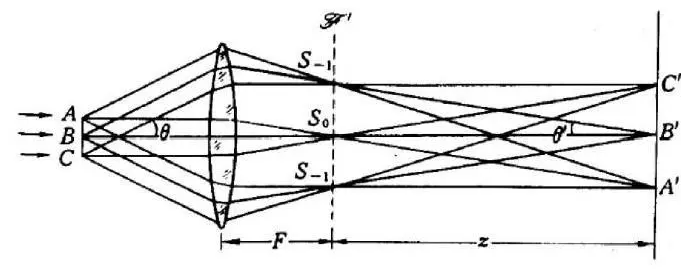
\includegraphics[width=0.8\columnwidth]{assets/1 阿贝尔/阿贝尔原理.png}
    \caption{阿贝成像原理}\label{阿贝成像原理}
\end{figure}

如图 \ref{阿贝成像原理} 所示,阿贝成像原理指出,光路中存在一个频谱面,
在这里不同物发出的同频率、同偏振方向的光汇聚在如图的三个点上,且满足:
\begin{equation}
    S_0=0\qquad S_{\pm 1} = \pm F\tan{\theta_i}\text{ , 其中}\sin{\theta_i} = f_i\lambda
\end{equation}
其中 $f_i$为余弦光栅的空间频率,$\lambda$为光的波长。我们以这三个点为次级波源,计算他们发射球面波的复振幅,形成干涉,在光屏上的结果即为经典理论计算的结果:
\begin{equation}
    U_{im}(x',y')=k{\rm e}^{ik\frac{{x^{'}}^2+{y^{'}}^2}{2z}}A_1(t_0+t_i\cos 2\pi f'_ix')
\end{equation}
从而可以得到以下结果:

\begin{enumerate}
\item 频谱面上的点是同波长的光汇聚的点,因此对于经过光栅、透镜的光,我们可以通过在频谱面上的滤波器来限制得到图像的结果。频谱面上的图像和像面上的图像都是光的信息经过透镜操作和光场传播后,在特定位置形成特定波前,但由于他们位置特殊,所以对他们进行的操作对人的帮助更大。
\item 对于通过光栅(也可以不通过,这样在频谱面形成的光斑是环形的)和透镜之后的光,我们可以在频谱面上加上遮挡光线的器具,或者用透明有色的物体限制通过的光波长范围,以实现“仅允许部分波长、偏振方向的光”通过的目的。
\end{enumerate}

本次实验便是通过放置在频谱面的滤波器滤掉多余的光波,仅保留需要的波长范围,以达到改变成像属性的目的。


在正式做实验之前,老师特意强调了光路搭建的三个要求:“平行、等高、准直”。
每个操作都有相应的细节对应:“平行”比较容易做到,因为本来就是一维光路,只需微调各透镜的角度,
保证透镜面垂直入射光面即可(当然,要保证凹凸面对准平行光);“等高”即将所需器材合至一起,
调节高度并固定(可利用白屏辅助检查),推荐为 90cm 左右,可根据实际情况进行调整;
“准直”可能是比较困难的步骤,也是最关键的步骤,进行准直镜的共焦调整之后,利用白屏远近移动以检查平行光质量。

根据讲义所写的过程,逐个安装并调整光学器件的位置。
讲义中给出的参考距离基本正确,可以先按照该距离进行粗糙地安装。
但注意光学仪器的位置并不等同于其下坐标的位置,
而且需要注意部分仪器的位置有偏差(尤其是后续实验中的白光 LED 灯,必要时可以用尺子辅助观察)

注意部件应当从激光器开始依次安装,
并在确认位置无误后拧紧螺丝。如果在安装过程中发现光路有问题,
应当从有问题的器件开始检查(就近调整原则)。

讲义的实物参考图如下:

\begin{figure}[H]\centering
    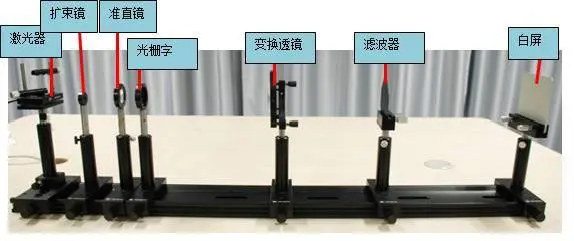
\includegraphics[width=0.8\columnwidth]{assets/1 阿贝尔/讲义实验台.png}
    \caption{讲义中的实验台搭建示例}\label{讲义中的实验台搭建示例}
\end{figure}

后续需要安装滤波器。
注意滤波器的位置应处在激光花样最清晰的位置,
即频谱面处,后者可以用光屏来辅助寻找位置。


\subsection{无滤波时“光”的像和频谱}

放置好光路图后,先观察没有滤波状态下的物像,
当放大倍数足够大时(可以通过将白屏放置尽可能远来实现),
可以观察到“光”字的像中间既有横向条纹,
也有竖向条纹,呈清晰的点阵结构。
这时候可以在变换透镜和白屏之间寻找频谱面,
从而帮助我们分析光路结构,进行下一步实验。我的实验图像如图 \ref{无滤波时的图像} 所示:

\begin{figure}[H]\centering
\begin{subfigure}[b]{0.5\columnwidth}\centering
    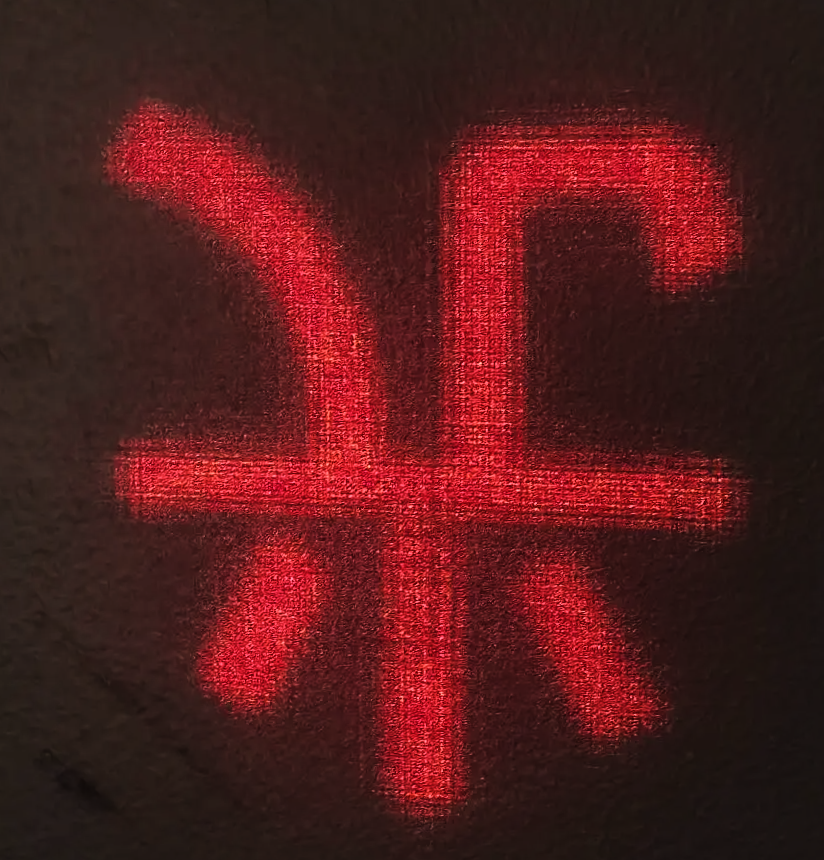
\includegraphics[height=215pt]{assets/1 阿贝尔/光 无滤波.png}
    \caption{“光”字的像}
\end{subfigure}\hfill
\begin{subfigure}[b]{0.5\columnwidth}\centering
    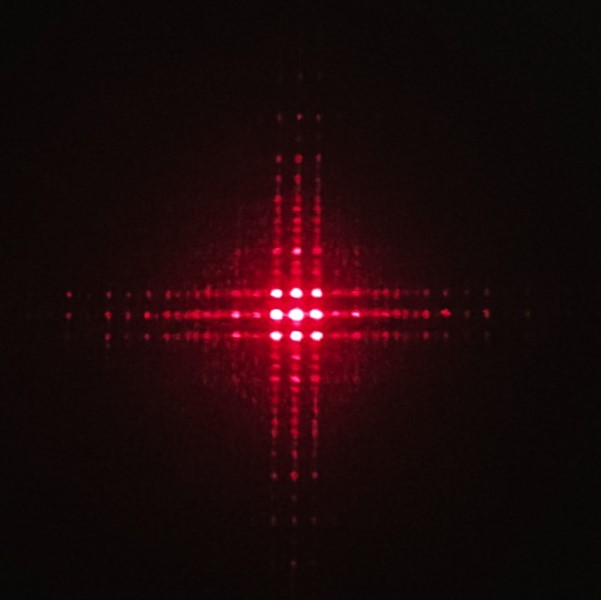
\includegraphics[height=215pt]{assets/1 阿贝尔/频谱面.jpg}
    \caption{频谱面}
\end{subfigure}
\caption{无滤波时的图像}
\label{无滤波时的图像}
\end{figure}

\subsection{狭缝滤波、低通滤波和自制高通滤波}

\subsubsection{狭缝滤波}

选择滤波器中的“缝”,在频谱面将狭缝水平放置,使包括 0 级光斑在内的一排光斑通过,我们可以观察到“光”的像中间充满竖向条纹,如图 \ref{狭缝滤波} (a) 所示;将滤波器旋转九十度,此时狭缝竖直,同样让 0 级处在内的一列点通过,可以观察到“光”像充满横向条纹,如图 \ref{狭缝滤波} (b) 所示:


\begin{figure}[H]\centering
\begin{subfigure}[b]{0.5\columnwidth}\centering
    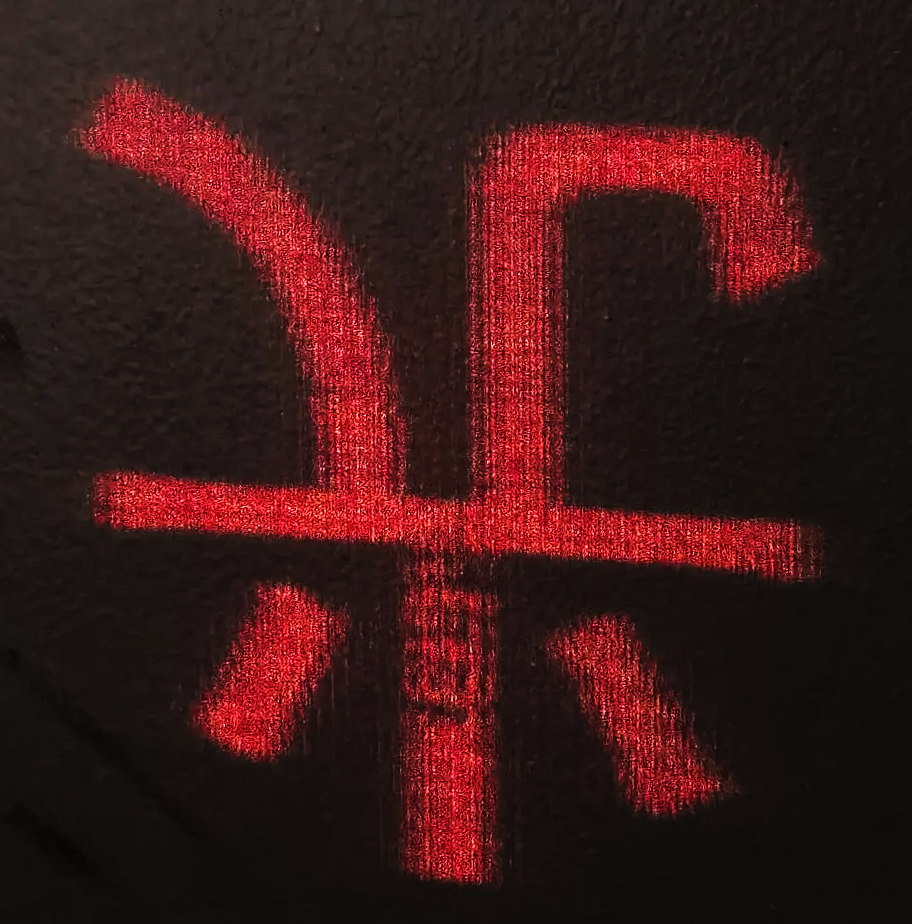
\includegraphics[height=215pt]{assets/1 阿贝尔/光 横向狭缝.png}
    \caption{横向狭缝,像有竖条纹}
\end{subfigure}\hfill
\begin{subfigure}[b]{0.5\columnwidth}\centering
    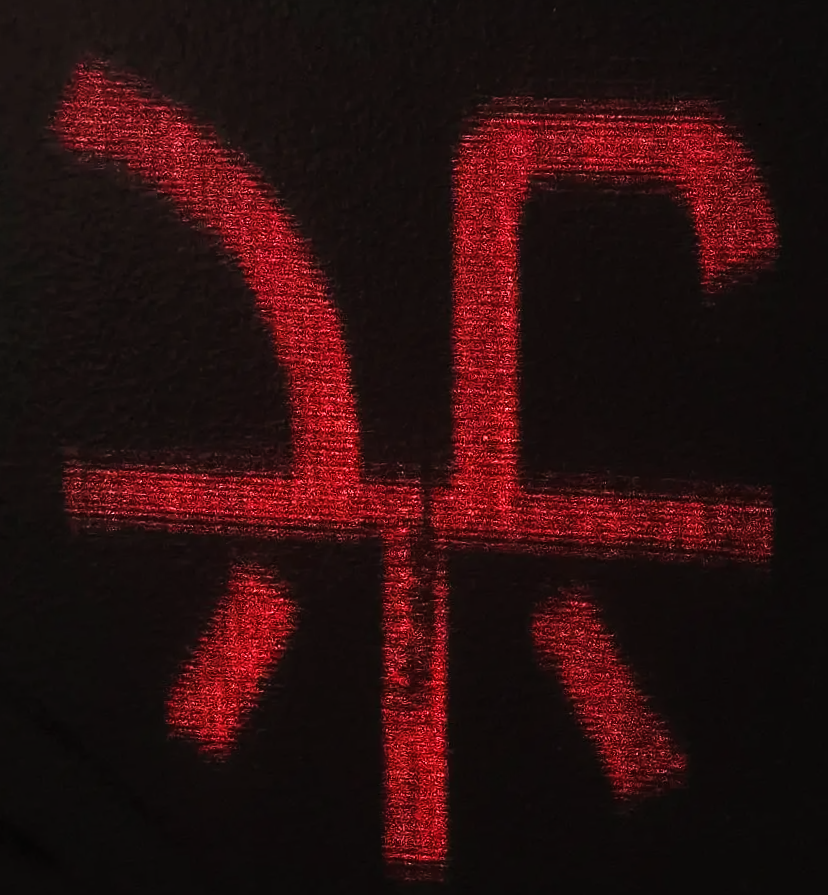
\includegraphics[height=215pt]{assets/1 阿贝尔/光 纵向狭缝.png}
    \caption{纵向狭缝,像有横条纹}
\end{subfigure}
\caption{狭缝滤波}\label{狭缝滤波}
\end{figure}


通过实验可以发现理论上的“光”字图像和
实际观察到的狭缝滤波图像仍存
在一定的差异。
首先是观察到的图像并不完全由条纹组成,
存在一些区域仍然是均匀填充的;并
且,在“光”字的某些部位出现了明显的暗斑(主要集中于“光”字上方那一短竖线)。
分析可能是因为:
\begin{enumerate}
\item 在调节准直时操作还不够细致,仪器之间也并没有做到严格的“等高共轴”,得到的光并非严格意义上的平行光;
\item 仪器本身存在缺陷和磨损。
\end{enumerate}

总的来说,上述三个小实验清晰地展示了滤波器对像图像的影响,且体现了衍射的特性:某一方向限制越强,则这一方面衍射现象越明显。


\subsubsection{低通滤波}

根据前面原理部分,频谱面上 $S_0$ 对应的就是物信息中的0频信息 $A_1t_0$ ,且位于面内的原点处;而正负两方向的衍射点 $S_{+1}$ 与 $S_{-1}$ ,代表了指定频率 $f'_i$ 的信息 $A_1t_i$ 。其位置由焦距 $F$ 以及衍射角 $\theta_i$ 决定:空间频率越大,衍射角就越高,衍射点距离中心也就越远(老师讲解时把其作为理论辅助实验的典型例子加以分析)。

故观察低通滤波(小孔滤波)的操作为:将滤波器中的“孔”放置在频谱面,
只让 0 级光斑通过。我们即可以观察到 “光”的像中间没有条纹,基本只剩下“光”字轮廓和实心填充。结果如图 \ref{低通滤波} 所示:

\begin{figure}[H]\centering
    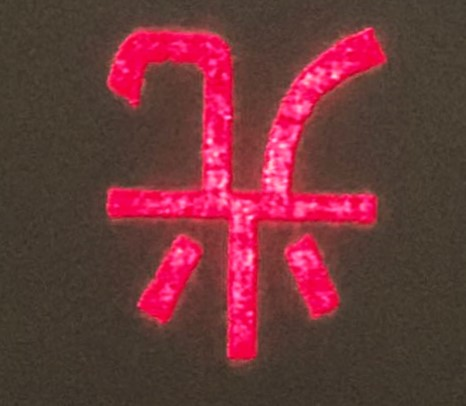
\includegraphics[height=215pt]{assets/1 阿贝尔/光 低通.jpg}
    \caption{低通滤波}\label{低通滤波}
\end{figure}

实际上,低通滤波器就是一个圆形光孔。由于图像的精细结构及突变部分主要由高频成分起作用,故经低通滤波后图像的精细结构消失,亮暗突变处变模糊。

理论上的“光”字图像和实际观察到的图像仍存在一定的差异。首先是在“光”字的某些部位仍然存在不那么明显的条纹;同时,在“光”字的某些部位也出现了明显的暗斑。除了上一实验中已经分析过的原因,还可能是因为实验过程中使用的小孔略大,导致实际透过小孔的并非只有 0 级光点,因此观察到了部分条纹。

在实验过程中,我还把小圆孔移到了中央以外的亮点上,此时在白屏上仍能看到不带网格的“光”字,只是较暗淡一些。这说明当物为“光”与网格的乘积时,其傅里叶谱是“光”的谱与网格的谱的卷积,因此每个亮点周围都是“光”的谱,再作傅里叶变换就还原成“光”字,这其实演示了傅里叶变换的乘积定理。

\subsubsection{自制高通滤波}

类似的,要完成高通滤波操作,只需要将 0 级光斑附近遮盖,周围留缝使光通过即可。我们采用自制的高通滤波器进行实验,制作的“器材”以及观察到的现象如下:

\begin{figure}[H]\centering
\begin{subfigure}[b]{0.5\columnwidth}\centering
    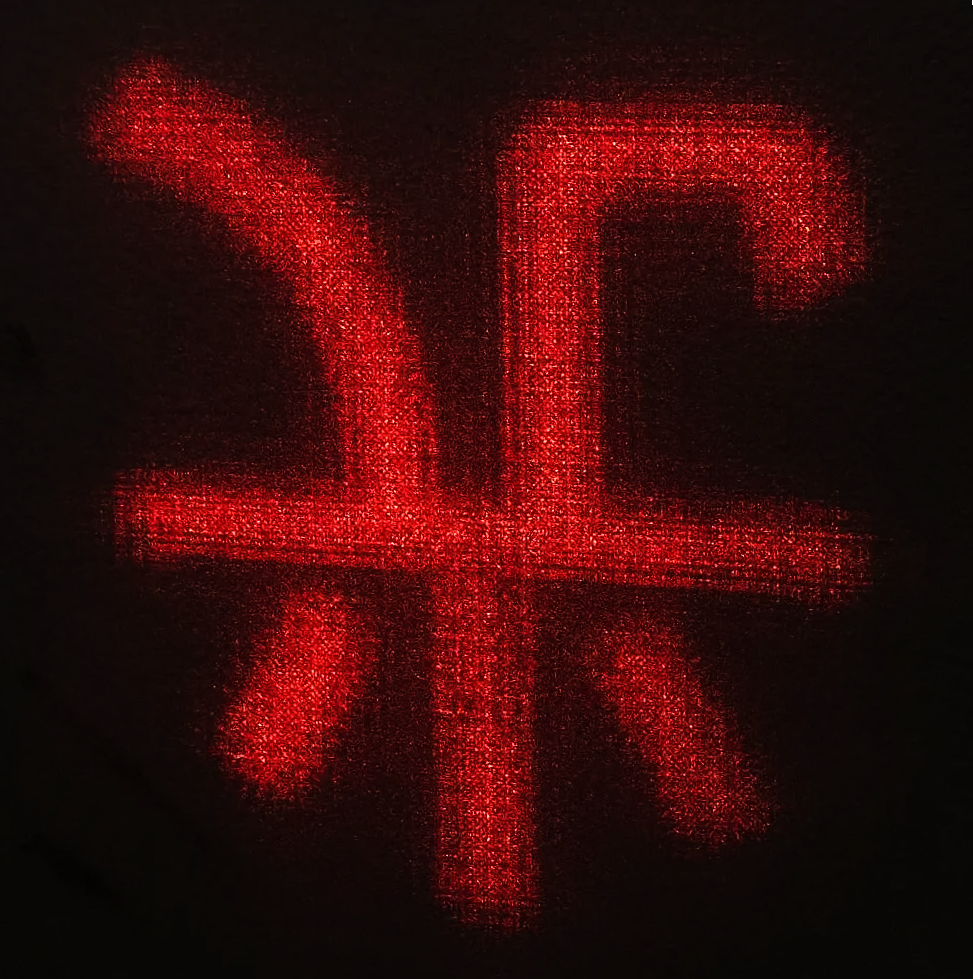
\includegraphics[height=215pt]{assets/1 阿贝尔/光 高通.png}
    \caption{“光”的像}
\end{subfigure}\hfill
\begin{subfigure}[b]{0.5\columnwidth}\centering
    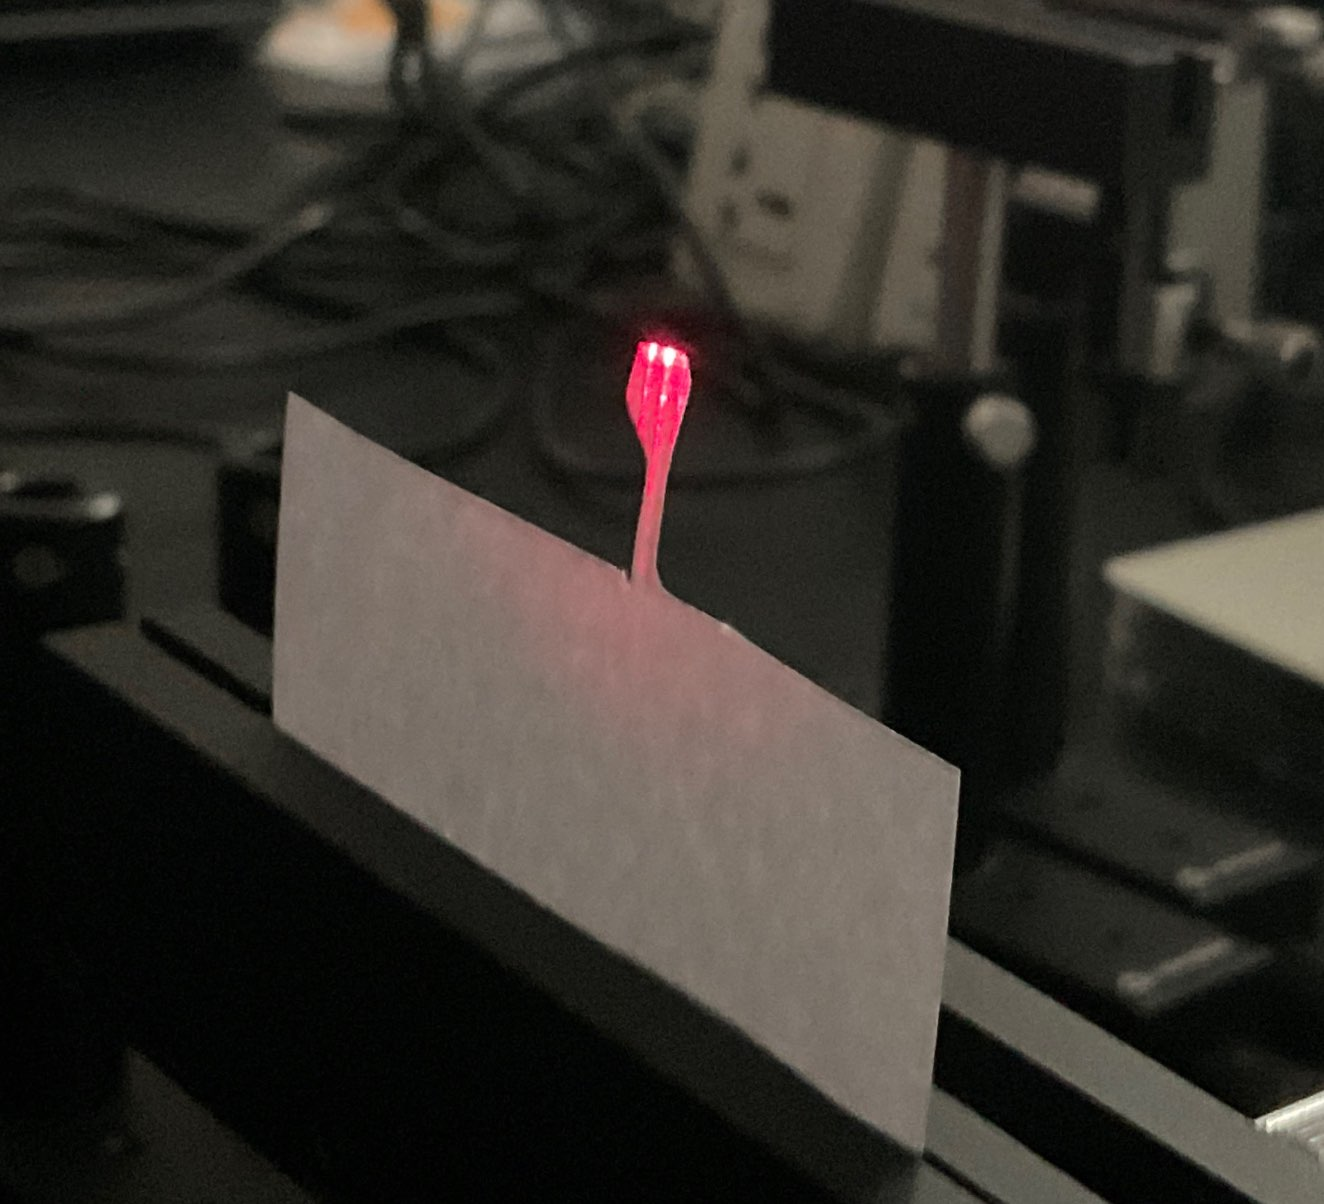
\includegraphics[height=215pt]{assets/1 阿贝尔/自制高通滤波器.jpg}
    \caption{自制高通滤波器}
\end{subfigure}
\caption{高通滤波}
\end{figure}

高通滤波的图像理论上整体变暗,实验图像清晰地显示了这一点。


\subsection{阿贝成像实验总结}

\begin{graybox}
\textbf{阿贝成像实验总结:}

上述实验简明扼要地展示了“频谱面”的特殊意义与重要性,实验图像清晰且符合预期(必要处我放大了局部细节辅助观察)。
我对图像的观察、思考与解释已经尽可能全面地叙述在上文对应图像附近了,实验整体是成功的。

本实验中现象都可以结合傅里叶变换和频谱面的观念加以解释——这是我觉得最美妙的地方。
比如在进行小孔滤波实验时,我移动小孔位置,
相当于“看到了”傅里叶变换的乘积定理(见对应实验);
假若利用小孔光栅(实验中我简单尝试了一下),
可观察到光屏上只有光亮而无条纹(只有直流分量),
这其实对应着“ $\delta(x)$ 的傅里叶变换就是1”的数学结果。

实际上,空间滤波有广泛的现实应用,
包括改良影像质量,去除高频噪声与干扰等。其中蕴含的原理都可以通过本次实验结果进行体会和理解。
\end{graybox}



\section{光学 4F 系统成像}

\subsection{实验目的}
\begin{enumerate}
\item 体会和掌握光学4F成像系统的组织和搭建。
\item 在前面阿贝成像实验的基础上,
进一步体会更为复杂的光学信息处理。
\end{enumerate}

\subsection{实验器材}

\begin{table}[H]
    \centering
    \caption{4F 成像系统:实验仪器与用具列表}
    \begin{tabular}{cc}\toprule
        组件名称 & 包含器件\\  \midrule
        光源组件& 半导体激光器、一维平移台、宽滑块、支杆和套筒\\ 
        准直镜组件& 凹透镜($\Phi 6$,$f=9.8$ mm)、凸透镜($\Phi 25$,$f=80$ mm)、透镜架、滑块、支
        杆和套筒\\ 
        变换透镜组件& 凸透镜($\Phi 40$, $f=175$ mm )、镜架、滑块、支杆和套筒\\ 
        滤波器组件& 滤波器(低通、方向滤波)、精密平移台、干板夹、滑块、支杆和套筒\\
        白屏组件& 白屏、干板架、滑块、支杆和套筒\\ 
        \bottomrule
    \end{tabular}
\end{table}


\subsection{实验原理}

光学4F图像处理系统使用两个透镜,依次实现傅里叶变换和反傅里叶变换的光学操作,把成像要素与频谱操作要素分离开,频谱面位于两个透镜的中间,对成像的干扰小。图 \ref{光路原理图} 为光路原理图:
\begin{figure}[H]\centering
    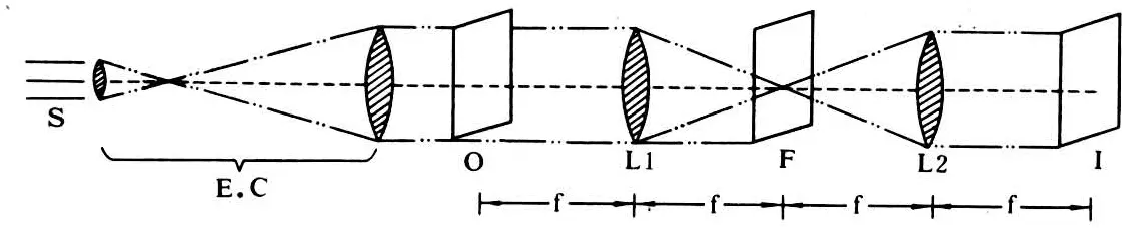
\includegraphics[width=0.8\columnwidth]{assets/2 透镜4F/光路原理图.png}
    \caption{光路原理图}\label{光路原理图}
\end{figure}

根据上一实验(阿贝变换),我们已经知道,透镜是对物像的光信息进行了一次傅里叶变换操作,而连续进行两次傅里叶变换操作会为原函数添加一个负号。一束平行光照射前焦面处的透明物体,产生待处理的图像,在第一个透镜的后焦面上得到物函数的频谱;而频谱面也是第二个透镜的前焦面,于是在第二个透镜的后焦面上得到第二次傅里叶变换,得到了原函数的倒像。

光学 4F 系统得到的像函数严格复制了原函数,同时消除了单透镜产生的附加相位因子对结果的影响,因此,与普通相干光学处理系统相比,较为复杂的光学 4F 系统的保真性更好、可控性更高。

\subsection{实验内容}

这一部分激光器、扩束器、准直镜不用移动。依次安装:物孔(即光栅字或者本实验中自制的“丁毅”字白纸),尽量靠近准直镜(减少不必要的光程);变换透镜 1,按照其焦距大致寻找其所在位置,固定后安装变换透镜2;随后就可以用光屏寻找最清晰像的位置。装置图如图 \ref{4F 讲义中的实验台搭建示例} 所示。

\begin{figure}[H]\centering
    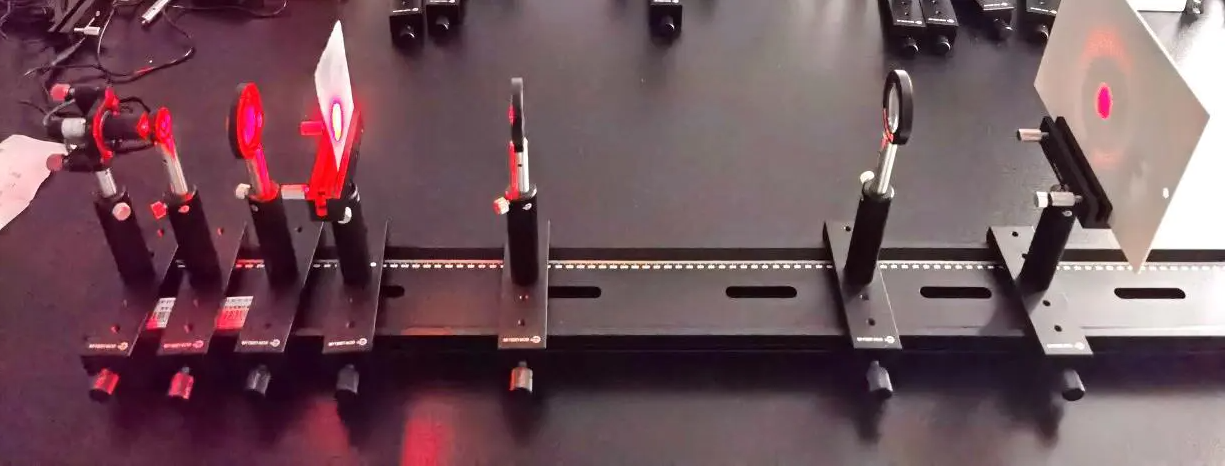
\includegraphics[width=0.80\columnwidth]{assets/2 透镜4F/讲义实验台.png}
    \caption{讲义中的实验台搭建示例}\label{4F 讲义中的实验台搭建示例}
\end{figure}

注意同上一部分,要求“平行、等高、准直”,透镜放置要求“凹凸面对准平行光”。


\subsection{实验现象与结果分析}

\subsubsection{观察“光”字}

仍使用“光”字作为被观察的物,图像如下:
\begin{figure}[H]\centering
    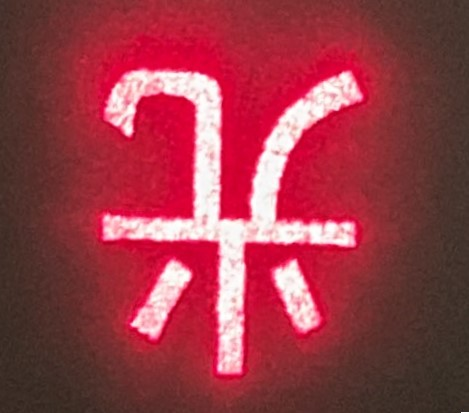
\includegraphics[height=215pt]{assets/2 透镜4F/光 透镜4F.jpg}
    \caption{4F 系统下的“光”字像}
\end{figure}

\subsubsection{观察自制“物”}
我们在白纸上写“丁毅”作为被观察的物,得到结果如图 \ref{4F 系统观察自制“物”的像} 所示:
\begin{figure}[H]\centering
\begin{subfigure}[b]{0.5\columnwidth}\centering
    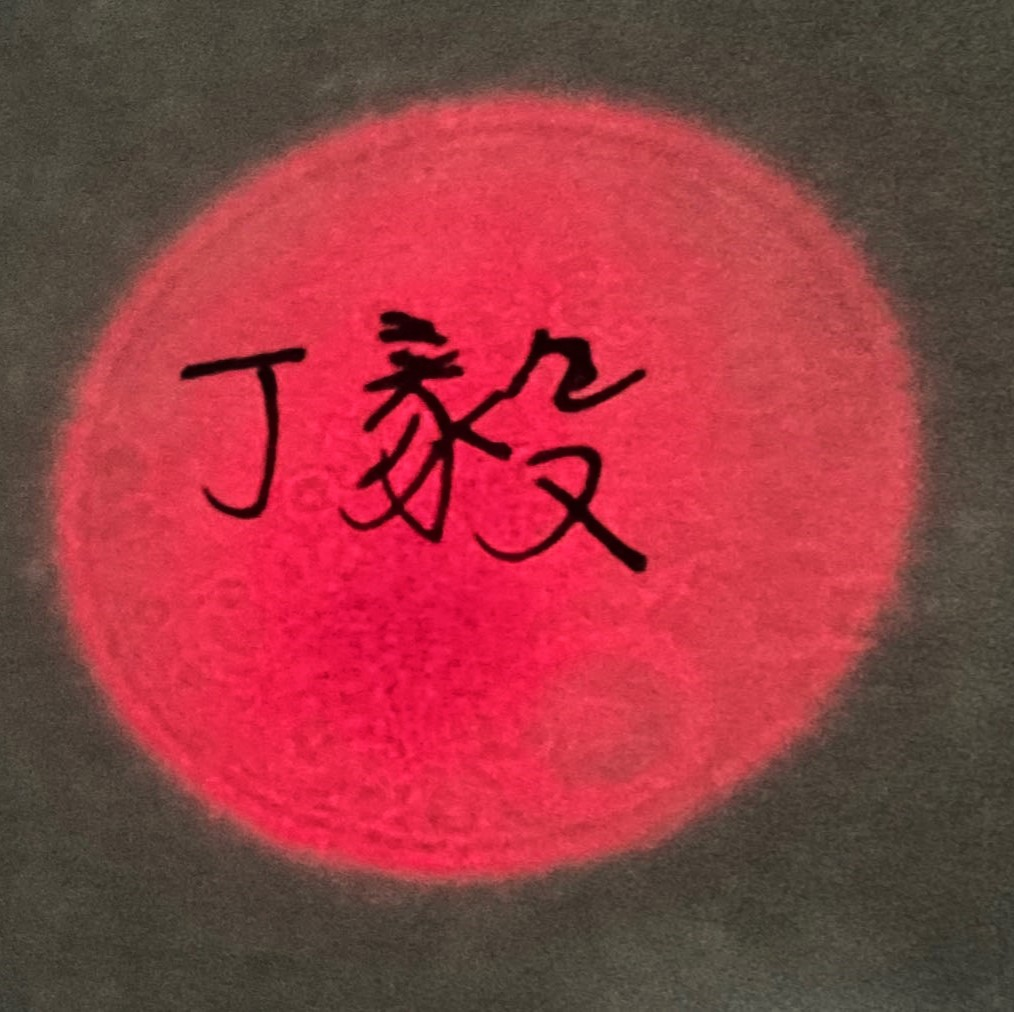
\includegraphics[height=215pt]{assets/2 透镜4F/透镜4F 自制物.jpg}
    \caption{自制“丁毅”作为被观察物}
\end{subfigure}\hfill
\begin{subfigure}[b]{0.5\columnwidth}\centering
    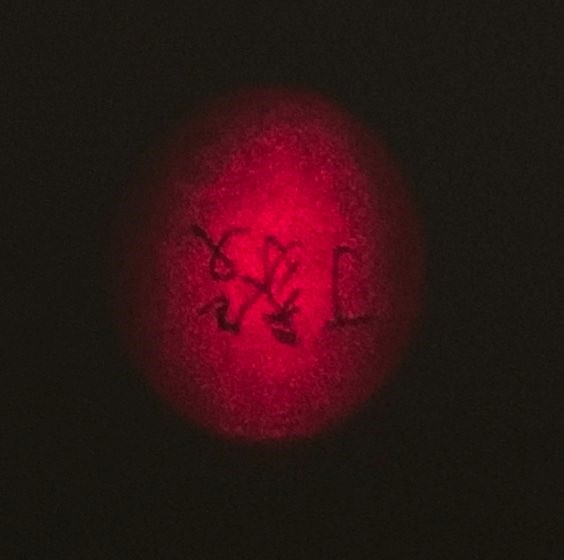
\includegraphics[height=215pt]{assets/2 透镜4F/透镜4F 自制物 像.jpg}
    \caption{4F 系统下的“丁毅”字像}
\end{subfigure}
\caption{4F 系统观察自制“物”的像}
\label{4F 系统观察自制“物”的像}
\end{figure}



\subsection{光学 4F 系统实验总结}

\begin{graybox}
\textbf{光学 4F 系统实验总结:}

很明显,与阿贝成像系统相比,4F 系统在白屏上的像清晰且明显,激光透过白纸黑字也能够在白屏上呈现清晰的像,说明 4F 系统保留调制物原有信息的能力更强。实际实验中,由于 4F 系统成像亮度过高,手机相机能力有限,图片无法将4F 系统成像的细节保留。

4F 系统的名字是很有物理直观意味的,原理同阿贝成像类似,但前者是单成像系统,虽然简单但可控参数太少,甚至会造成空间信息利用不充分的现象。相比阿贝成像,后者更加可控、保真、稳定性好,在实验图像中也显示出这一点。

\end{graybox}



\section{假彩色编码}

\subsection{实验目的}
\begin{enumerate}
\item 在基本空间滤波的基础上,进一步体会光栅衍射的色散效果和选频滤波操作,掌握$\theta$调制假彩色编码的选频滤波和色散选区滤波的原理;
\item 利用提前预制分区信息的光栅图案,
实现该图像的假彩色编码。
\end{enumerate}



\subsection{实验器材}

\begin{table}[H]
    \centering
    \caption{实验仪器与用具列表}
    \begin{tabular}{cc}
        \toprule
        组件名称 & 包含器件\\ \midrule
        光源组件& 白光LED、一维平移台、宽滑块、支杆和套筒\\ 
        准直镜组件& 凸透镜($\Phi 40$,$f=80$ mm)、透镜架、滑块、支杆和套筒 \\ 
        调制物组件& 天安门光栅($100$线/mm)、干板架、滑块、支杆和套筒\\ 
        变换透镜组件& 凸透镜($\Phi 76$,$f=175$ mm)、镜架、滑块、支杆和套筒\\ 
        滤波器组件& 滤波器、干板架、滑块、支杆和套筒\\ 
        白屏组件& 白屏、干板架、滑块、支杆和套筒\\ 
        \bottomrule
    \end{tabular}
\end{table}

\subsection{实验原理}

使用白光光源来照明一个分区事先预制了不同取向光栅的天安门图案,然后分别使用颜色滤波器和自制的空间选色滤波器,来实现天安门图像的选区假彩色编码。

天安门光栅中,天空、天安门、草地三个区域预制了不同方向的光栅刻线(空间频率为100线/nm),分别对应蓝、红、绿色。一个白光光源照射透明的天安门产生衍射,不同颜色的光会分散传播,经透镜汇聚在频谱面上,形成彩色衍射花样。天安门光栅上不同的区域方向不同,所以衍射花样会延三个不同方向展开,呈现出彩色的带状花样。选用三个不同方向不同颜色(红、绿、蓝)的彩色滤片,或一张在不同部位戳出孔洞(在实验中需要自制,根据实际情况)的白纸,来选取颜色通过,实现不同区域的彩色编码。最终在光屏上,我们会得到一个绿草地、
红天安门和蓝天组合图像(自制滤片颜色自定)。



\subsection{光路布置和调节}

这部分实验需要更换光源并重新布置光路。要求同前面一样。值得一提的是准直操作,需要耐心检验,而且因为讲义上提供的参数不太准确,这一部分的光路搭建我自行调整了不少距离。注意LED灯和凸透镜的间距需要用尺子测量,并校准到产生了平行光(或者在光屏移动时,投射上的光并没有产生变化)。由于白光是多种波长的光复合而成的,不可能完全准直,所以搭建时差不多即可。图 \ref{假彩示意} 是讲义中的实验台搭建示例:
\begin{figure}[H]\centering
    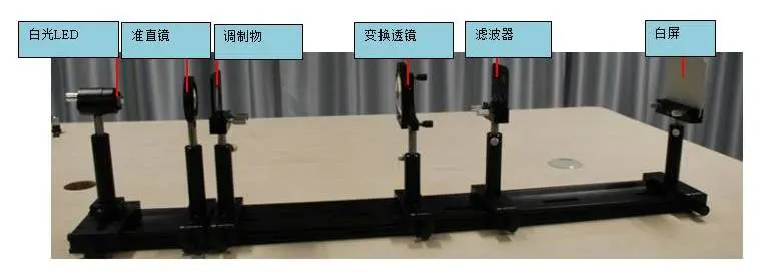
\includegraphics[width=0.8\columnwidth]{assets/3 假彩编码/讲义图.png}
    \caption{讲义中的实验台搭建示例}
    \label{假彩示意}
\end{figure}

\subsection{实验现象与结果分析}

\subsubsection{无滤波器}

在  $\theta$  调制之前,观察天安门图像,可以看到呈现无彩色、放大、倒立(相较于天安门光栅本身)的像,将白屏至于频谱面上,可以看到分散的彩色衍射图样。
\begin{figure}[H]\centering
\begin{subfigure}[b]{0.5\columnwidth}\centering
    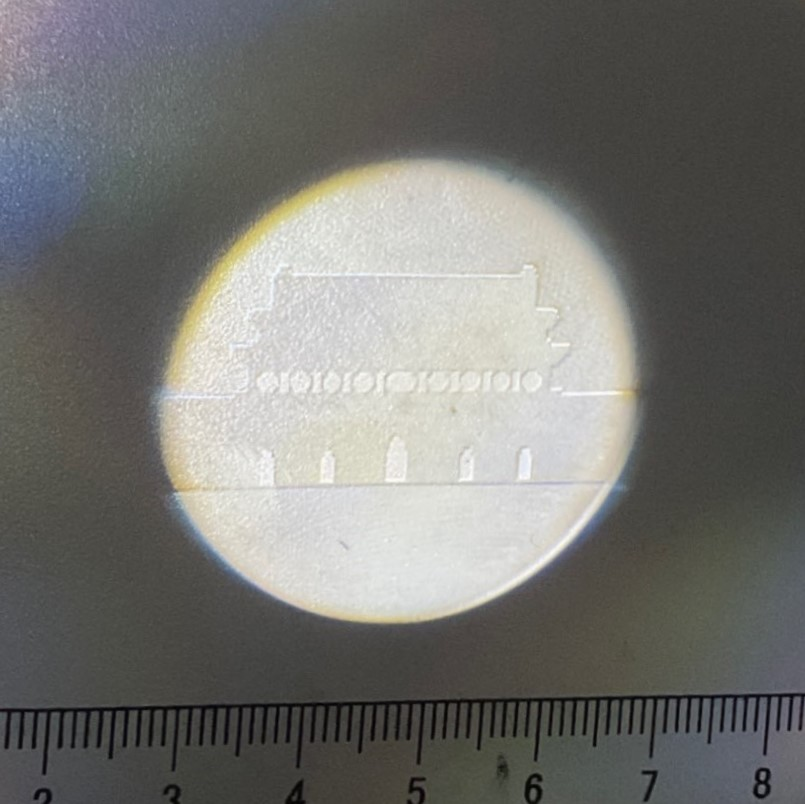
\includegraphics[height=215pt]{assets/3 假彩编码/天安门 无滤波器.jpg}
    \caption{天安门的像}
\end{subfigure}\hfill
\begin{subfigure}[b]{0.5\columnwidth}\centering
    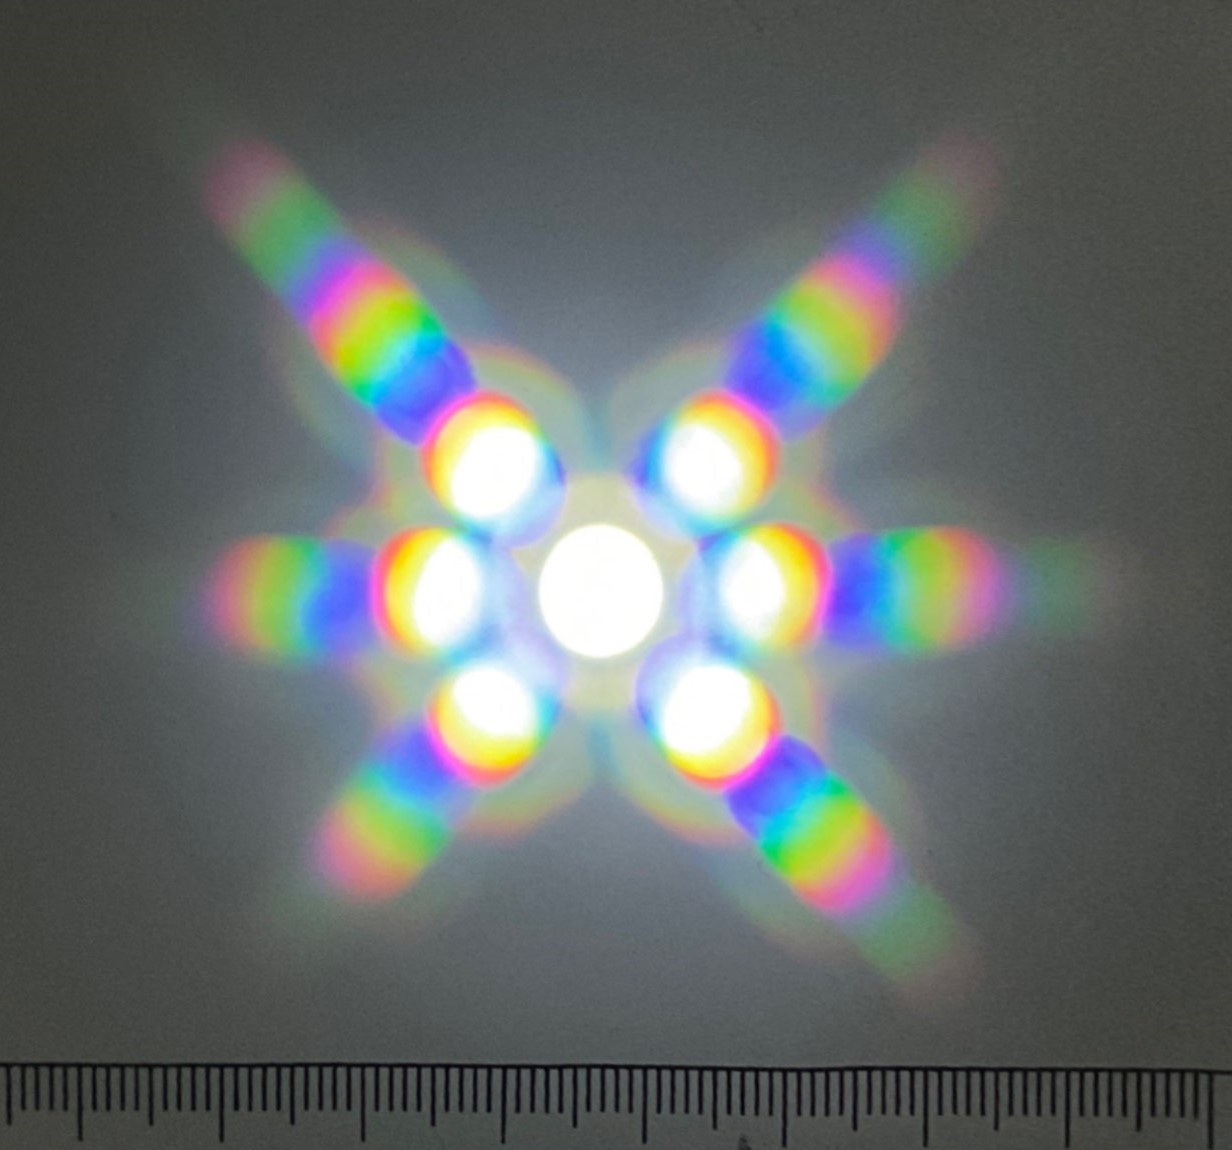
\includegraphics[height=215pt]{assets/3 假彩编码/彩色频谱面 (2).jpg}
    \caption{彩色频谱面}
\end{subfigure}
\caption{无滤波器时天安门的像}
\end{figure}

\subsubsection{$\theta$ 调制滤波器}

使用 $\theta$ 调制滤波器:安装 $\theta$ 调制滤波器到滤波器支架上,然后调整 $\theta$ 调制滤波器的正反和左右位置。调整好后,在白屏上观看经假彩色编码得到的像,可以看到蓝天、红天安门和绿草地,如图 \ref{调制滤波器下天安门} 所示。
\begin{figure}[H]\centering
\begin{subfigure}[b]{0.66\columnwidth}\centering
    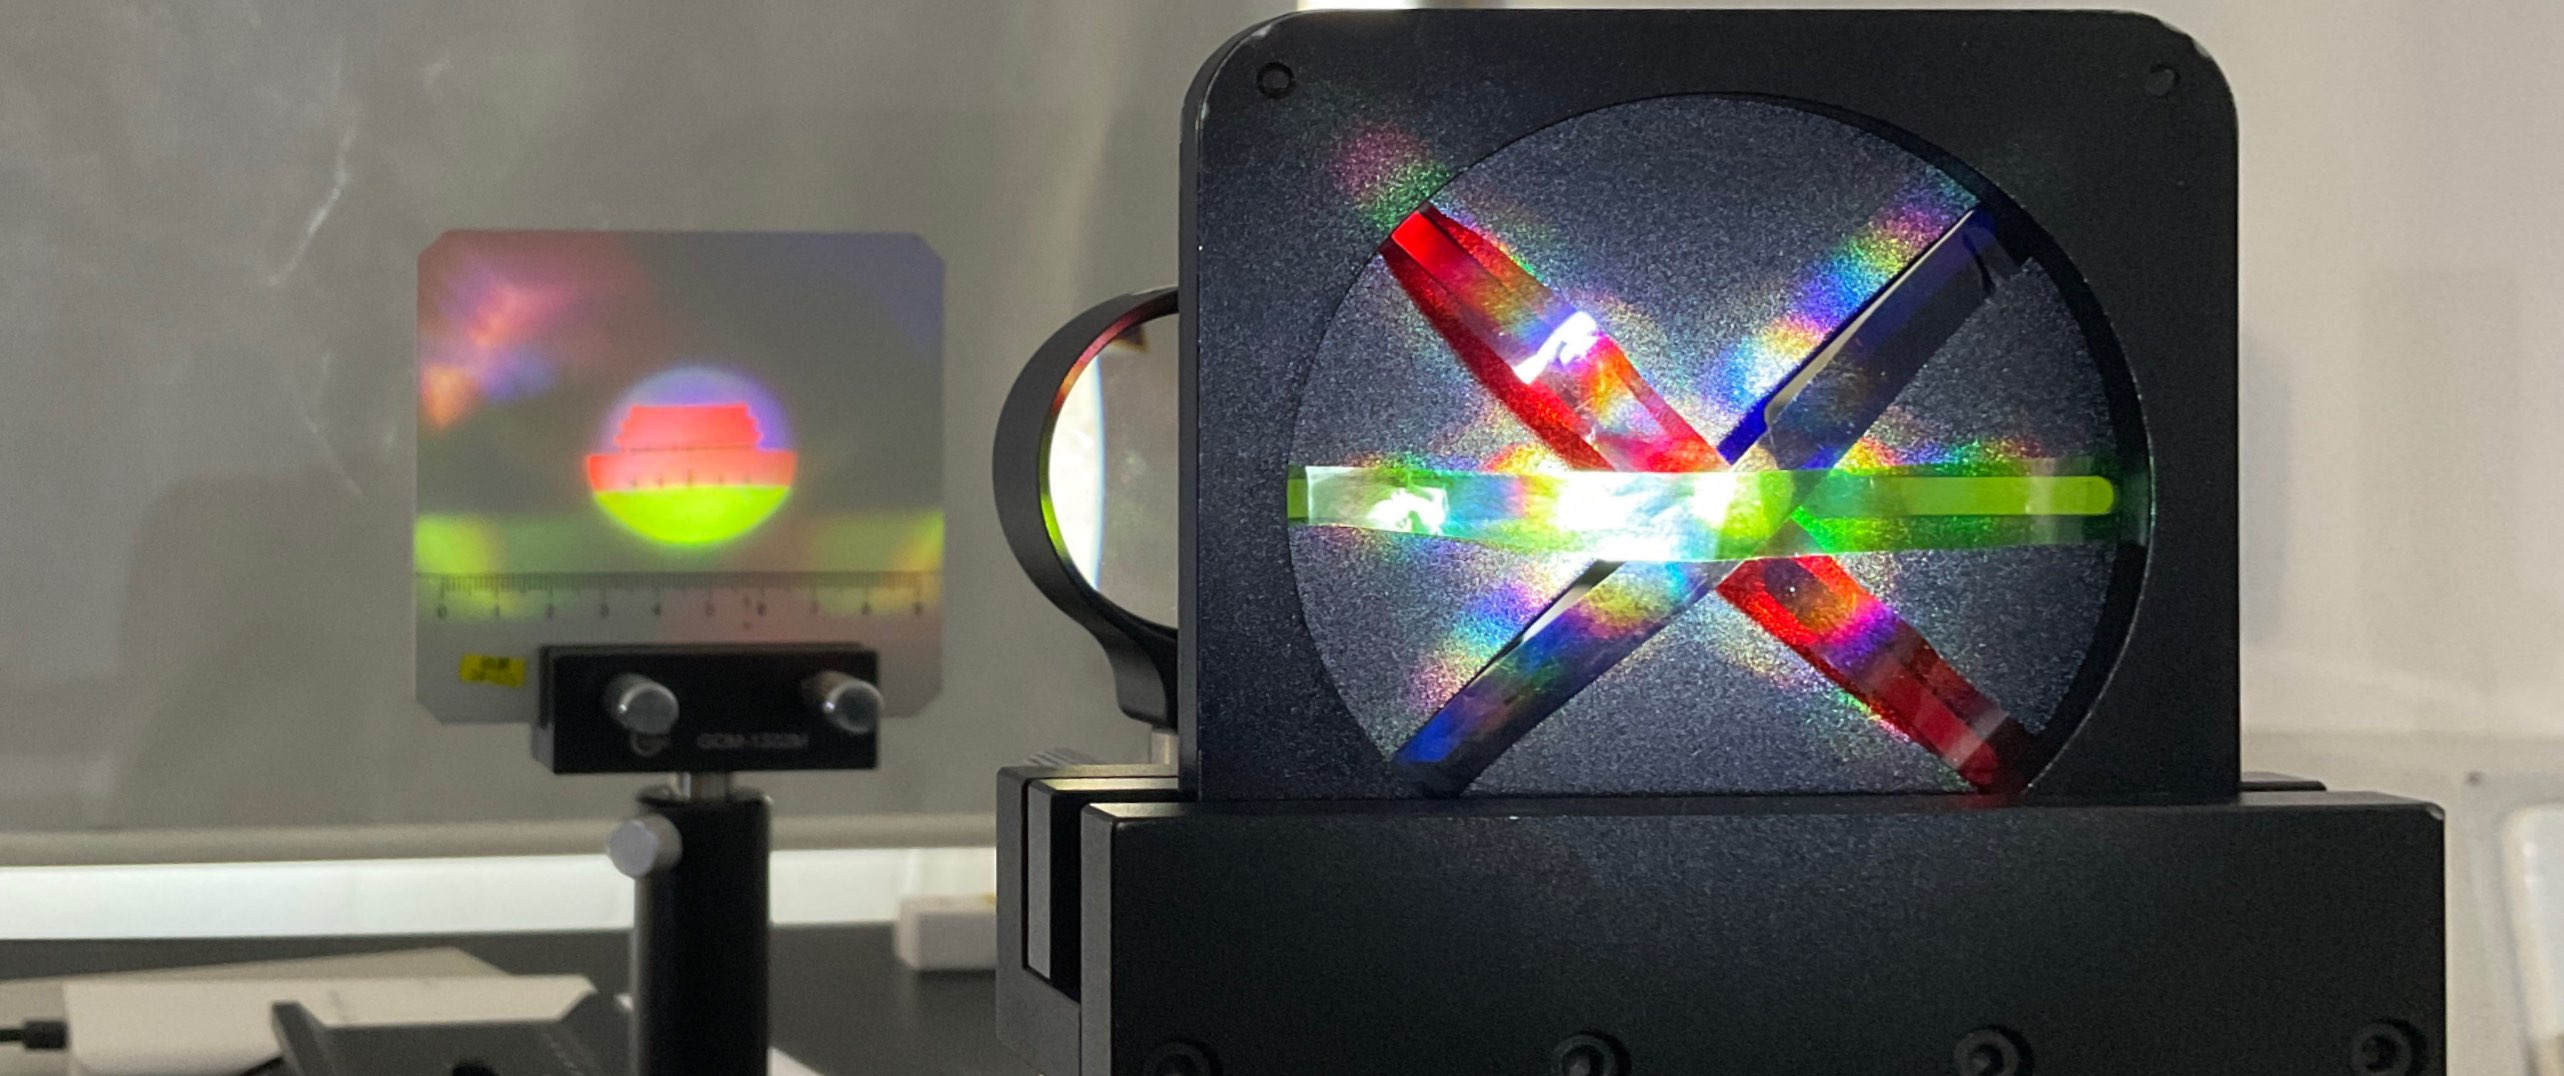
\includegraphics[height=130pt]{assets/3 假彩编码/天安门 红色 实验台.jpg}
    \caption{实验台示意}
\end{subfigure}\hfill
\begin{subfigure}[b]{0.33\columnwidth}\centering
    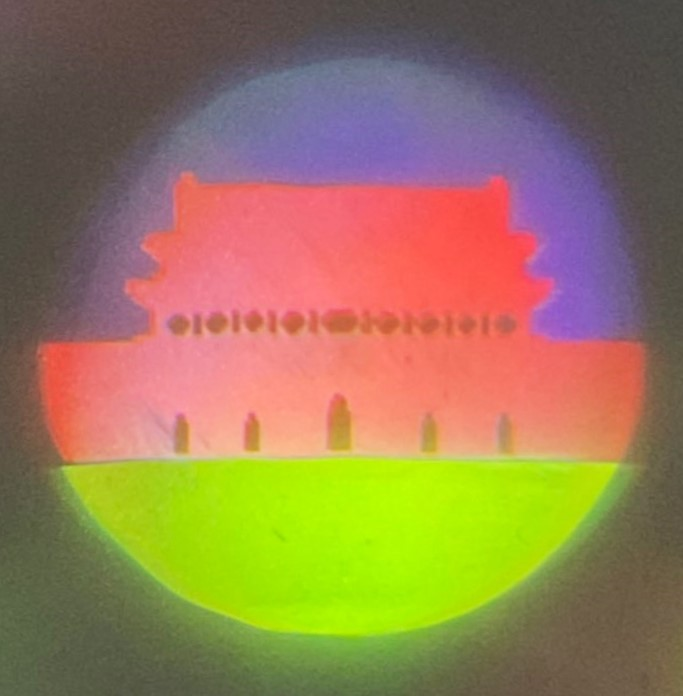
\includegraphics[height=130pt]{assets/3 假彩编码/天安门 红色.jpg}
    \caption{天安门图像放大}
\end{subfigure}
\caption{$\theta$ 调制滤波器下天安门}
\label{调制滤波器下天安门}
\end{figure}


\vspace*{-7mm}
\subsubsection{自制滤波器}

使用自制滤波器:利用老师给的纸片,先将纸片放在频谱面上,在各个方向上标记需要滤波通过的颜色,用铅笔画出,然后用裁纸刀挖去要通过的部分,重新放回频谱面,即可观察滤波效果。

\begin{figure}[H]\centering
\begin{subfigure}[b]{0.66\columnwidth}\centering
    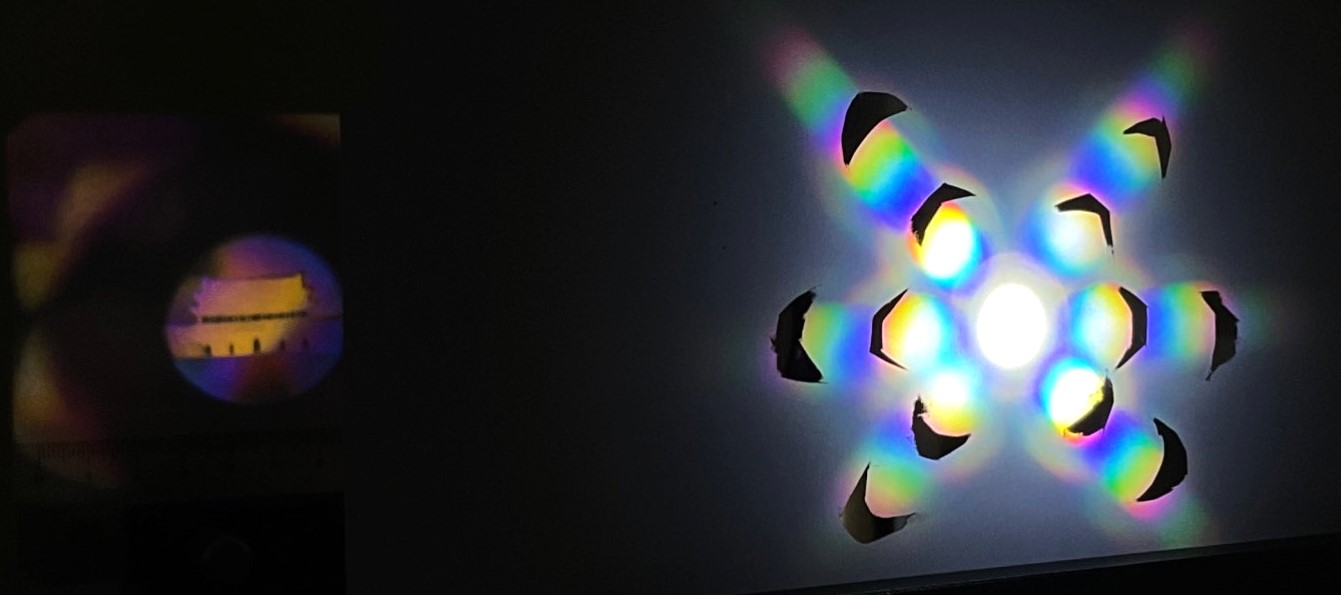
\includegraphics[height=130pt]{assets/3 假彩编码/自制滤波器 天安门暗.jpg}
    \caption{自制滤波器}
\end{subfigure}\hfill
\begin{subfigure}[b]{0.33\columnwidth}\centering
    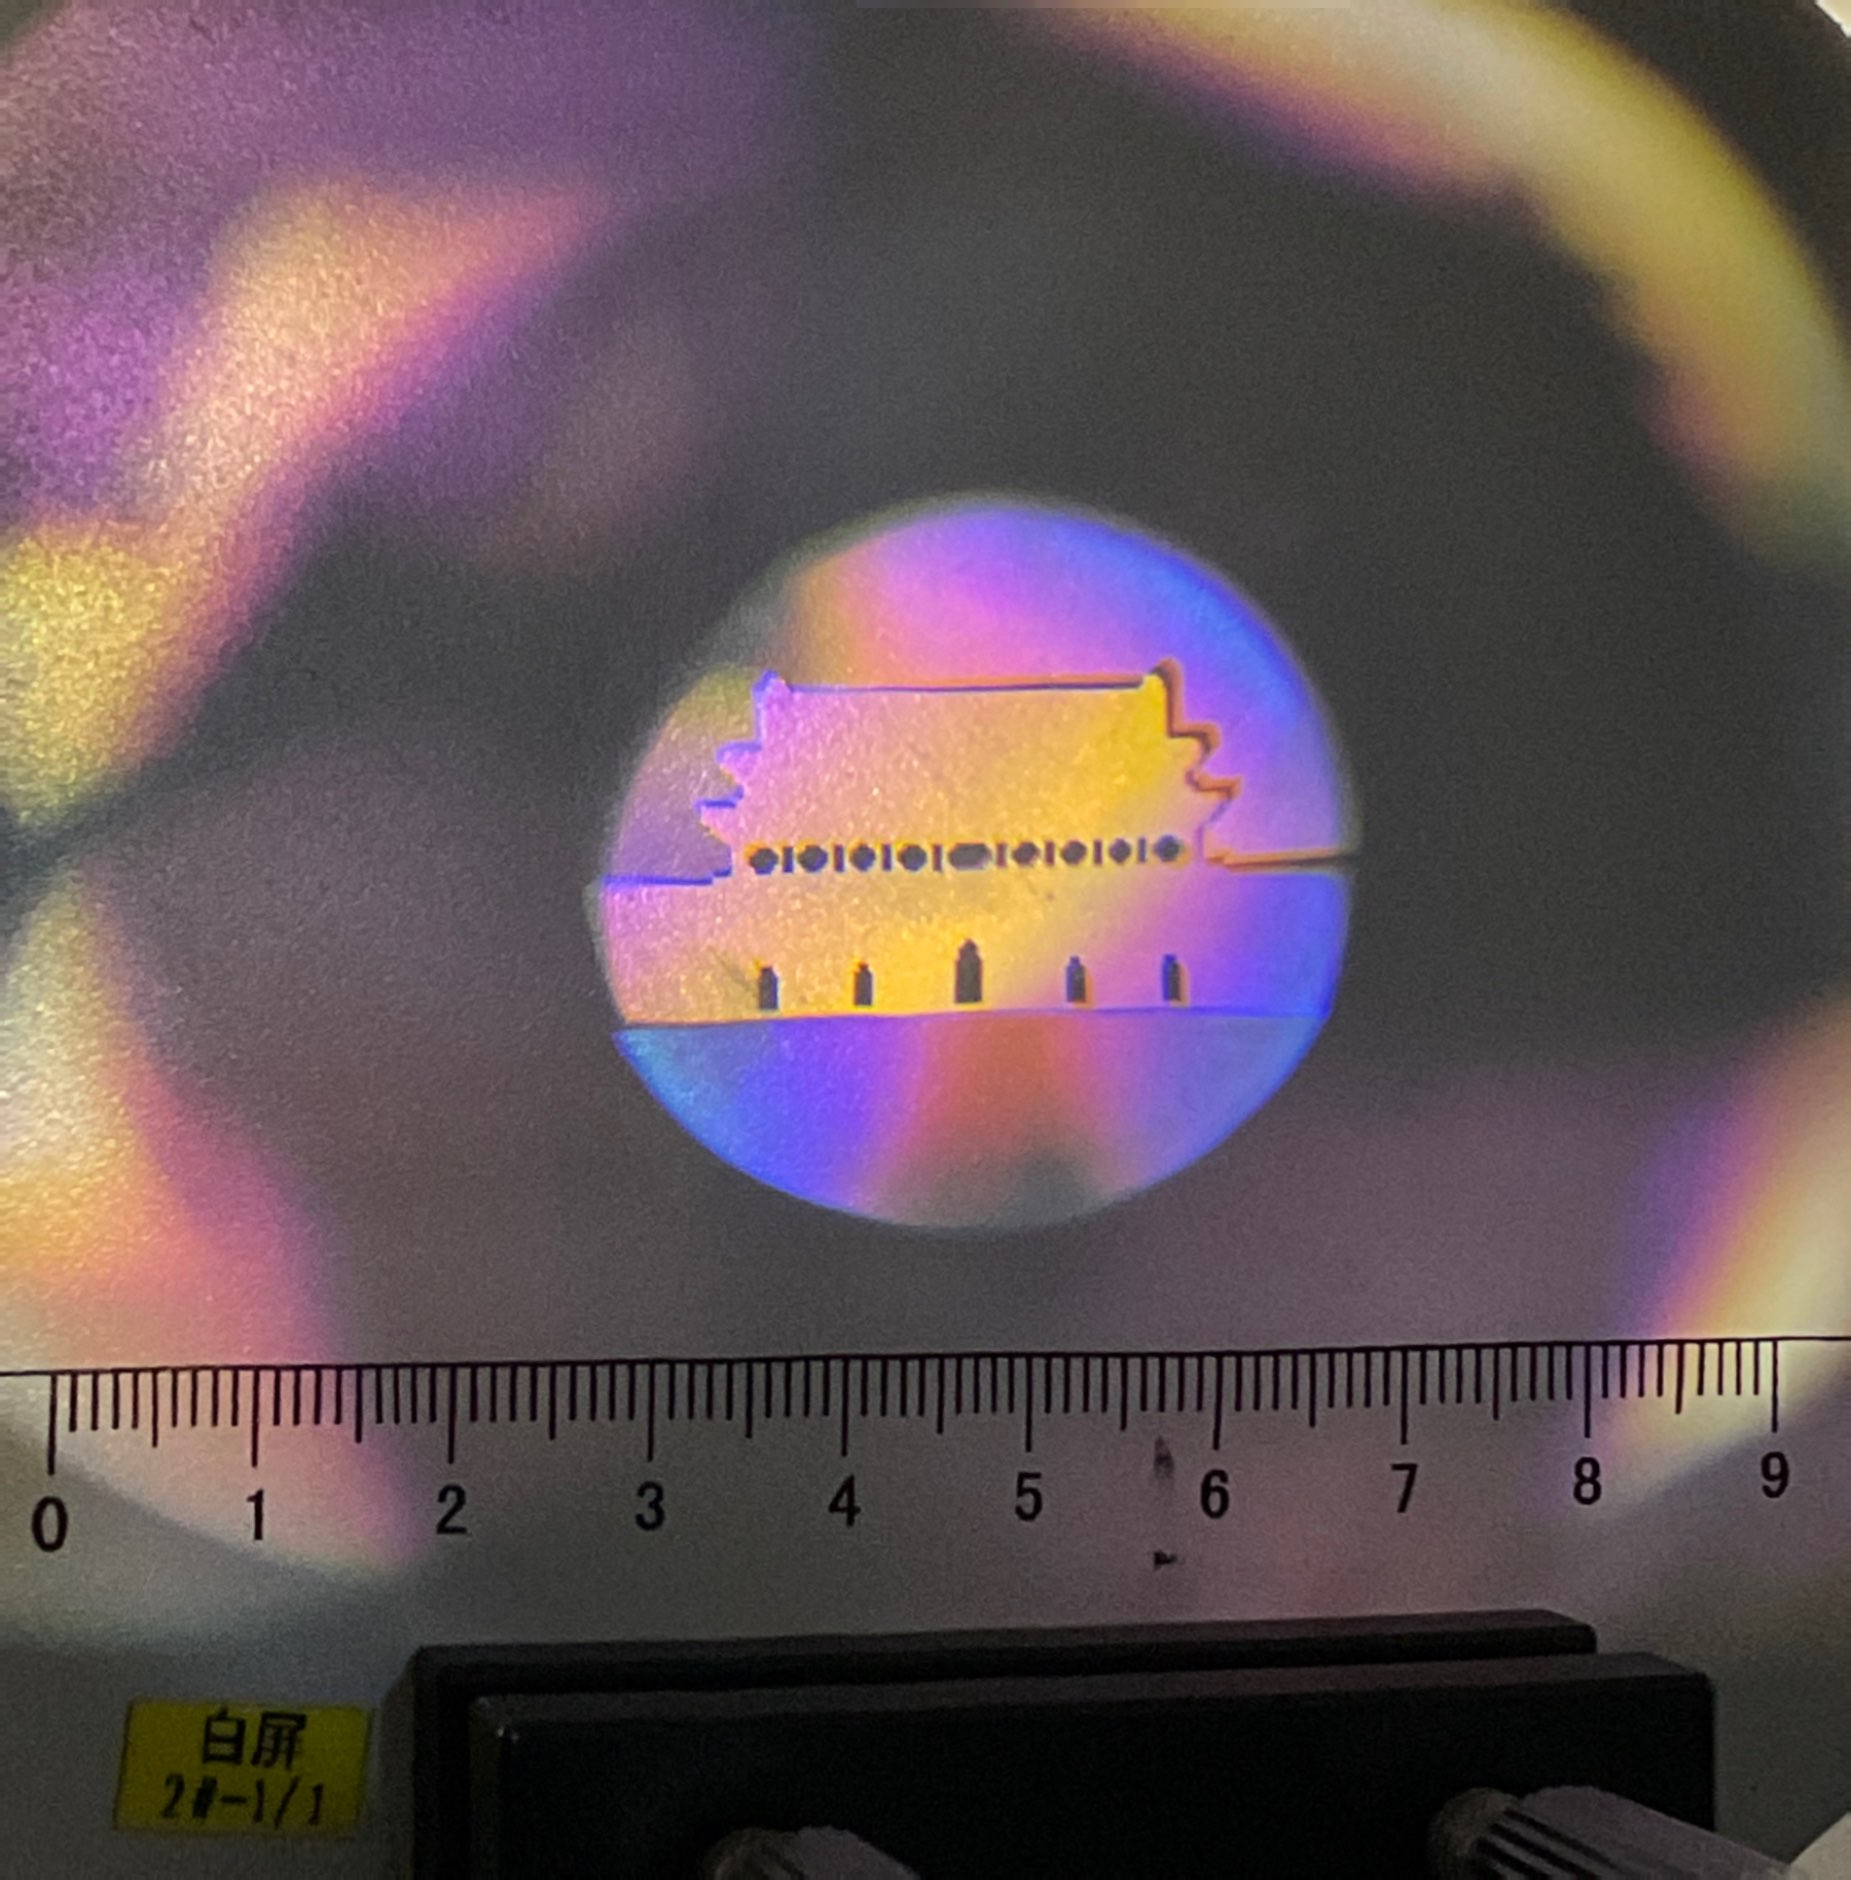
\includegraphics[height=130pt]{assets/3 假彩编码/天安门 自制 暗.jpg}
    \caption{天安门图像放大}
\end{subfigure}
\caption{自制滤波器及对应的天安门图像}
\end{figure}

\vspace*{-7mm}
\subsection{假彩色编码实验总结}
\vspace*{-5mm}
\begin{graybox}
\textbf{假彩色编码实验总结:}

本次实验在基本空间滤波的基础上,利用 $\theta$ 调制滤波器和自制的滤波器进行了选频滤波的操作,动手体会了光栅衍射的色散效果及相应原理在实验中的具体体现。整体上,实验是比较成功的。

实验开始时,我得到的结果是一个颜色不对的天安门,表现为天空为红色,天安门为蓝色,如图 \ref{调制器正反错误} 所示。检查后发现是 $\theta$ 调制器正反放置错误,纠正后便能得到预期结果。
\end{graybox}

\begin{figure}[H]\centering
\begin{subfigure}[b]{0.66\columnwidth}\centering
    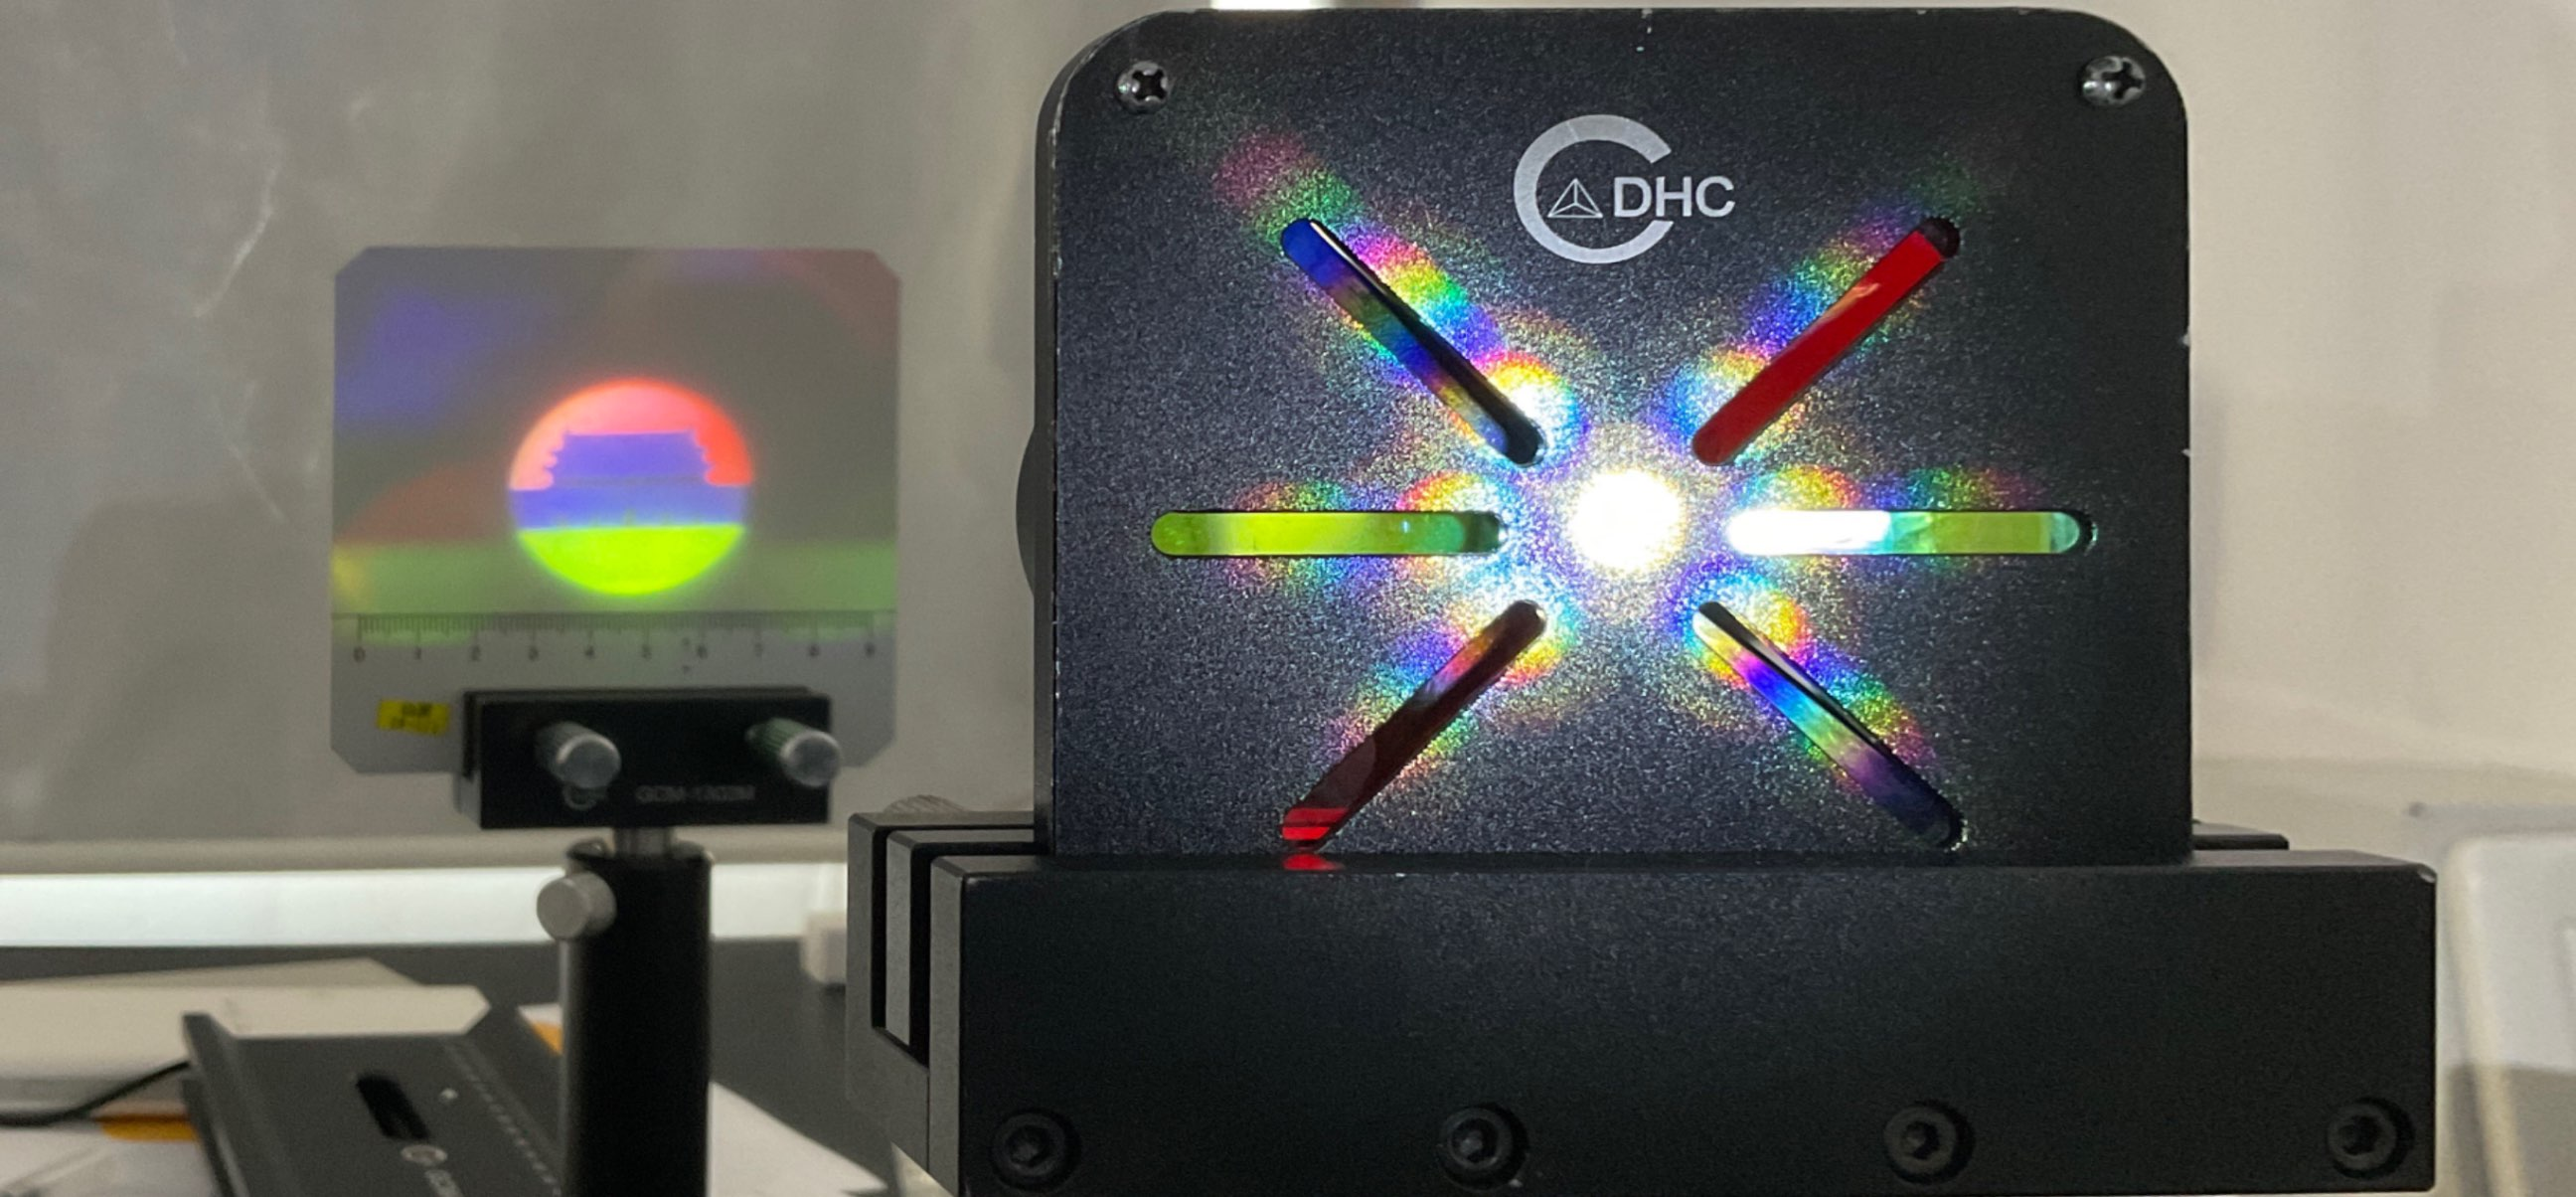
\includegraphics[height=130pt]{assets/3 假彩编码/天安门 蓝色 实验台.jpg}
    \caption{$\theta$ 调制器正反错误}
\end{subfigure}\hfill
\begin{subfigure}[b]{0.33\columnwidth}\centering
    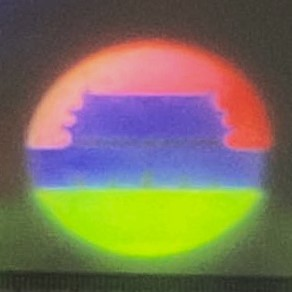
\includegraphics[height=130pt]{assets/3 假彩编码/天安门 蓝色.jpg}
    \caption{蓝色的“天安门”}
\end{subfigure}
\caption{$\theta$ 调制器正反错误时得到的结果}
\label{调制器正反错误}
\end{figure}



\section{光栅、夫琅禾费衍射与光谱仪测量光谱}

\subsection{实验目的}

\begin{enumerate}
\item 将透射光栅放入光路中,根据衍射光斑图样,代入光栅方程计算光栅常数 d;
\item 通过实验测量与计算,熟悉光栅的结构与衍射原理,熟悉光学测量的操作;
\item 使用手持式光栅光谱仪和 SpectraSmart 软件测量激光或白光的光栅衍射光的光谱和波长,判断与经验值是否一致;
\item 通过实验,了解LED灯的光谱,初步了解光栅光谱仪与相应软件的测量方法。
\end{enumerate}


\subsection{实验器材}

待测量光栅、衍射分划板、半导体激光器、平移台、白屏、干板架、宽滑块、滑块、支杆和套筒;光栅光谱仪测光谱实验器材: OTO SE1040 便携式光栅光谱仪(测量波长范围 $350 \ \mathrm{nm} \ \sim \ 1020 \ \mathrm{nm}$),另外还有白光LED、一维平移台、白屏、干板架、宽滑块、滑块、支杆和套筒等。

\subsection{实验原理}

\subsubsection{测量光栅常量}

光栅由大量等宽等间距的平行狭缝构成,光线射入光栅后会发生衍射,光会产生分解,分别射向不同方向,其原理即为衍射的原理。根据光栅方程,我们可以计算出光栅的缝间距,也即光栅常数 $d$,判断与已知光栅刻缝数(据老师介绍,有 100、300、600 三种规格)是否一致。

\subsubsection{夫琅禾费衍射}
用给定的衍射分划板进行夫琅禾费衍射实验。板上有 3 条透光狭缝(单缝)、3 条挡光狭缝(单丝)、3 各透光小孔(小孔)和 3 个挡光小孔(小屏)共十二项,依次观察现象并拍照记录。我在实验中使用的分划板参数如下:
\begin{center}
\noindent\begin{minipage}{0.49\columnwidth}
\begin{table}[H]\centering
    %\renewcommand{\arraystretch}{1.5} % 调整行间距为 1.5 倍
    %\setlength{\tabcolsep}{1.5mm} % 调整列间距
    \caption{分划板参数}
    \label{分划板参数}
\begin{tabular}{cccccccccc}\toprule
    序号 & 1 & 2 & 3  \\
    \midrule
    单缝 & $a = 0.1$ mm &  $a = 0.2$ mm &  $a = 0.3$ mm   \\
    单丝 & $a = 0.1$ mm &  $a = 0.2$ mm &  $a = 0.3$ mm   \\
    小孔 & $\Phi = 0.2$ mm & $\Phi = 0.3$ mm & $\Phi = 0.4$ mm \\
    小屏 & $\Phi = 0.2$ mm & $\Phi = 0.3$ mm & $\Phi = 0.4$ mm \\
    \bottomrule
\end{tabular}
\end{table}
\end{minipage}\hfill\begin{minipage}{0.43\columnwidth}
\begin{figure}[H]\centering
    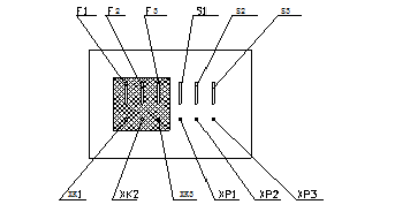
\includegraphics[width=0.95\columnwidth]{assets/4 衍射实验/分划板.png}
    \caption{分划板示意图}\label{分划板示意图}
\end{figure}
\end{minipage}\end{center}

\subsubsection{光栅光谱仪测光谱}

光栅光谱仪是用光栅作为色散元件的分光仪器,利用光栅将成分复杂的光分解为沿不同方向的单色光,可用于产生单色光,或利用光探测器测量得到光的波长组成。光栅光谱仪可用于光源的光谱分析或材料的光谱特性测量等。

在本次实验,我们使用手持式光栅光谱仪和 SpectraSmart 软件测量激光或白光的光栅衍射光的光谱和波长,判断与经验值是否一致。导出数据,再转至 Matlab 软件里绘制图像,作进一步的数据分析。

\subsection{实验结果与数据处理}

\subsubsection{测量光栅常数}

按照激光器、光栅、光屏的顺序在一维平移台上放置好实验器材,搭建光路。将复合透射光栅放入光路中,得到衍射光斑图样如图 \ref{复合光栅实验} 所示。

\begin{figure}[H]\centering
\begin{subfigure}[b]{0.95\columnwidth}\centering
    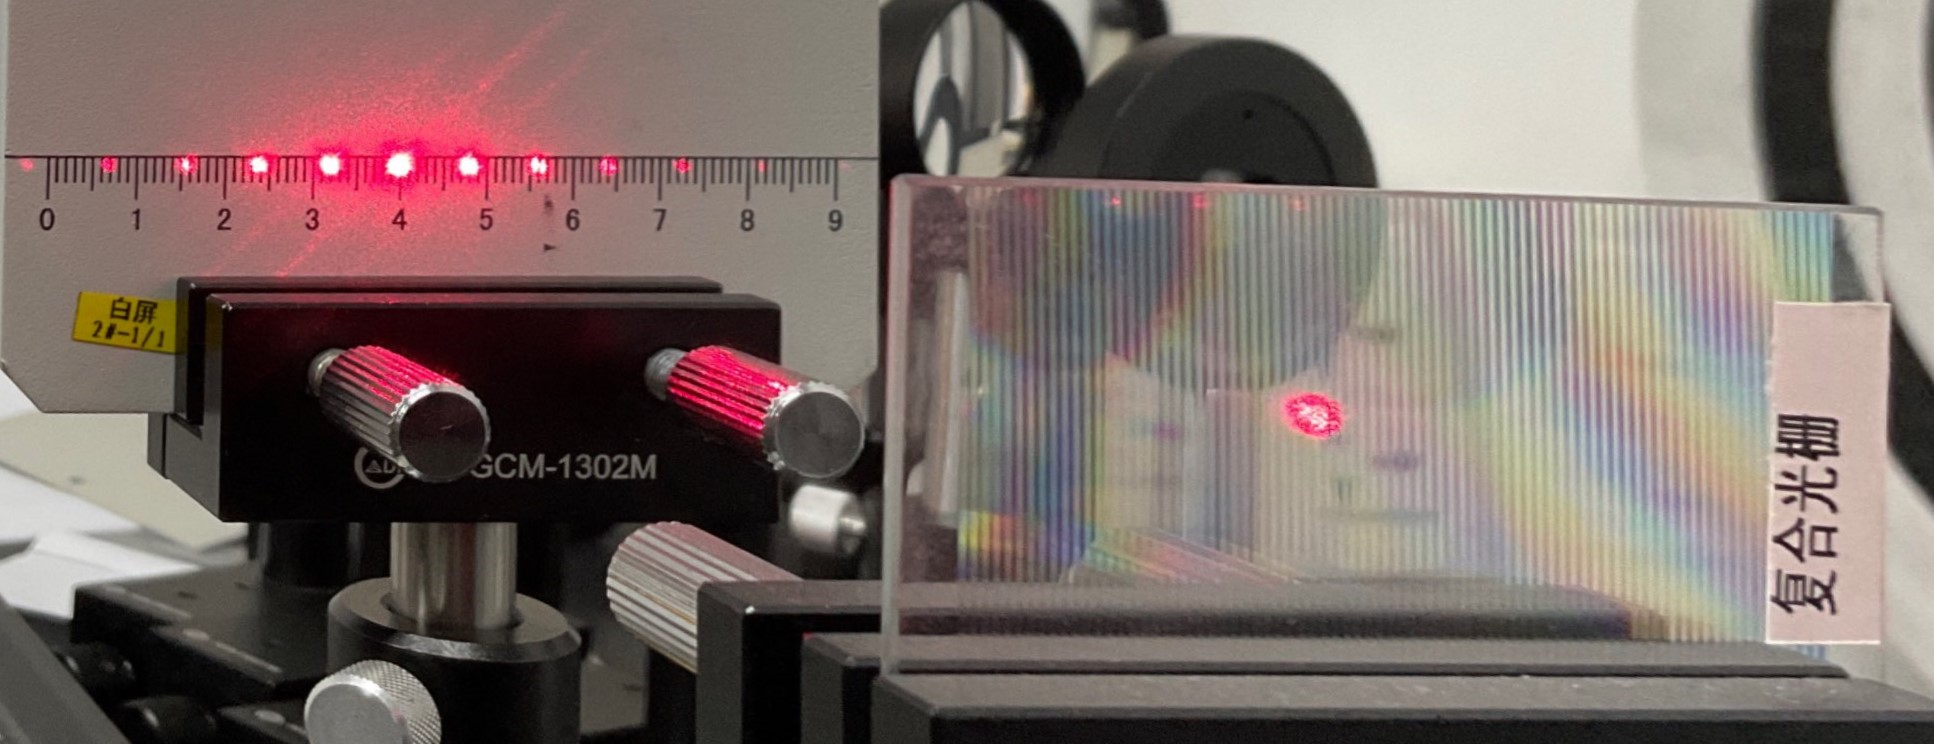
\includegraphics[width=\columnwidth]{assets/4 衍射实验/复合光栅实验台搭建.jpg}
    \caption{复合光栅实验台示意图}
\end{subfigure}
\begin{subfigure}[b]{0.95\columnwidth}\centering
    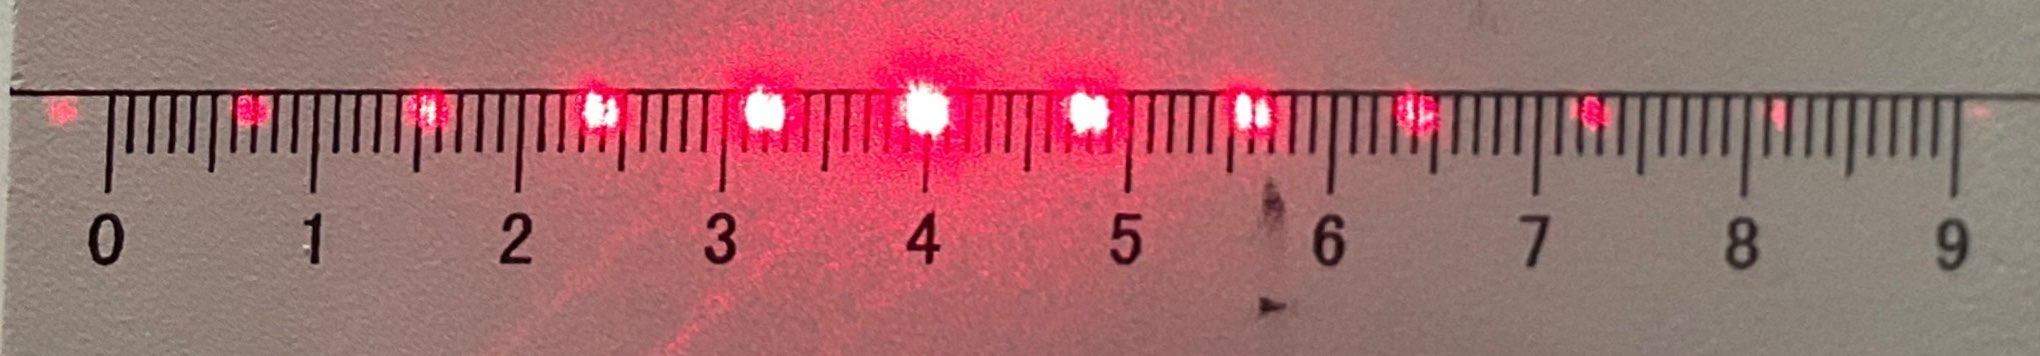
\includegraphics[width=\columnwidth]{assets/4 衍射实验/复合光栅衍射点.jpg}
    \caption{读取衍射光斑位置}
\end{subfigure}
\caption{测量复合光栅的光栅常数}
\label{复合光栅实验}
\end{figure}

由光栅方程可得到光栅常数的计算公式:
\begin{gather}
    d\sin{\theta} = m\lambda \quad \Longrightarrow \\ 
    N_{\text{mm}} = \frac{1 \times 10^{-3}}{d} = \frac{\sin \theta}{m\lambda} \times 10^{-3} = \frac{\tan \theta}{\sqrt{1 + \tan^2 \theta}}\cdot \frac{1}{m\lambda}\times 10^{-3},\quad \tan \theta = \frac{x}{l}
    ,\ m=0,\pm 1, \,\cdots
\end{gather}
其中 $N_\text{mm}$ 表示光栅每毫米中的刻缝数,$\theta$ 表示从干涉图样中心到第 $m$ 级极大之间的夹角,$\lambda$表示光的波长。

实验中我固定了光屏到光栅的距离 $l=12.0$ cm,由后文对红色激光器的拟合结果可知,激光器的主波长在 ${\color{red} \lambda = 656.3226\ \mathrm{nm}}$。从图 \ref{复合光栅实验} 中读取衍射光斑位置(以向右为正),做中心化和平均化后,代入上式计算,得到光栅常数:
\begin{table}[H]\centering
    %\renewcommand{\arraystretch}{1.5} % 调整行间距为 1.5 倍
    %\setlength{\tabcolsep}{1.5mm} % 调整列间距
    \caption{复合光栅衍射光斑位置}
    \label{复合光栅衍射光斑位置}
\begin{tabular}{cccccccccc}\toprule
    级数 $m$ & 0 & 1 & 2 & 3 & 4 & 5 \\
    \midrule
    原始位置 (cm) & 4.0 & (4.8, 3.2)  & (5.6, 2.4)  & (6.42, 1.67) & (7.26, 0.69) & (8.15, -0.21)  \\
    作中心化 (cm) & 0.0 & (0.8, -0.8) & (1.6, -1.6) & (2.42, 2.43) & (3.26, -3.31) & (4.15, -4.21)  \\
    作平均化 (cm) & 0.0 & 0.8 & 1.6 & 2.425 & 3.285 & 4.180  \\
    光栅常量 $d \ \mathrm{(\mu m)}$ & NaN & 9.867 & 9.932 & 9.940 & 9.943 & 9.976  \\
    刻线密度 (每 mm) & NaN & 101.3511 & 100.6850 & 100.6006 & 100.5738 & 100.2397  \\
    \bottomrule
\end{tabular}
\end{table}
待测光栅的规格可能是 100、300、600 条每毫米,由上表可知,所测的光栅刻线密度为 $100$ 条 / mm。

\subsubsection{夫琅禾费衍射}
我们依次对单缝、单丝、小孔和小屏做了衍射实验。前三项实验现象都较为明显,但是最后一项由于屏直径过小,大部分光线未被阻挡而直接射向观察屏,导致屏上实验现象被覆盖,无法观察到衍射。因此,我们仅在图 \ref{小孔衍射现象} 中给出一个图像(观察不到衍射现象)。各项实验现象如下所示:

\begin{figure}[H]\centering
\begin{subfigure}[b]{\columnwidth}\centering
    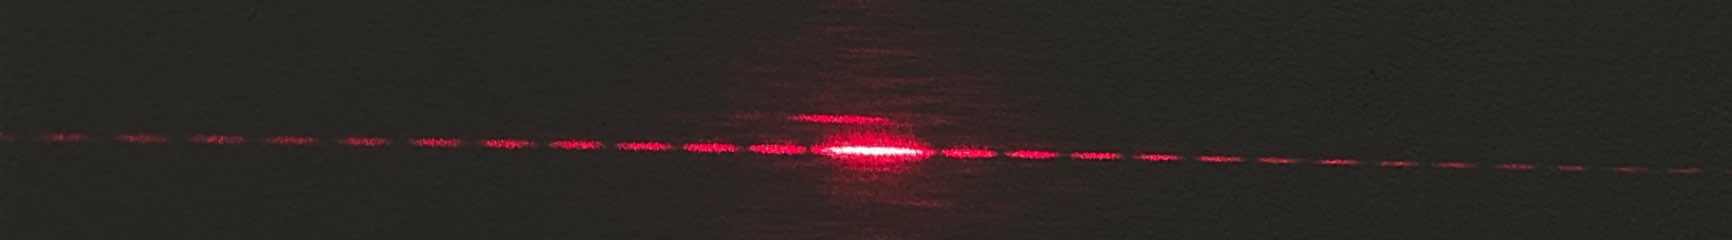
\includegraphics[width=\columnwidth]{assets/4 衍射实验/狭缝 1.jpg}
    \caption{单缝 1 (宽 0.1 mm)}
\end{subfigure}\hfill
\begin{subfigure}[b]{\columnwidth}\centering
    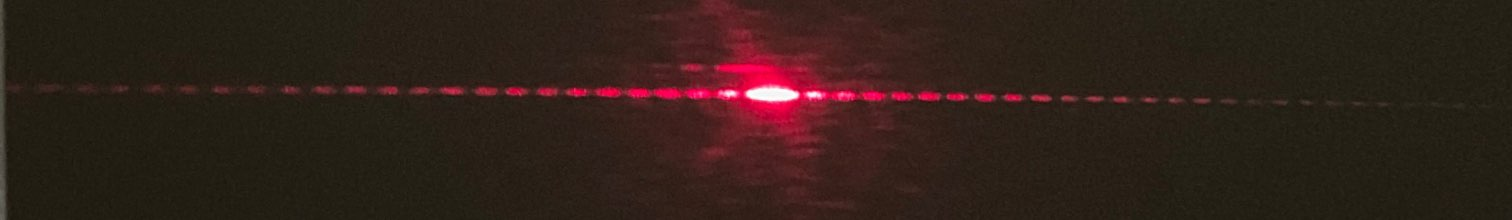
\includegraphics[width=\columnwidth]{assets/4 衍射实验/狭缝 2.jpg}
    \caption{单缝 2 (宽 0.2 mm)}
\end{subfigure}
\begin{subfigure}[b]{\columnwidth}\centering
    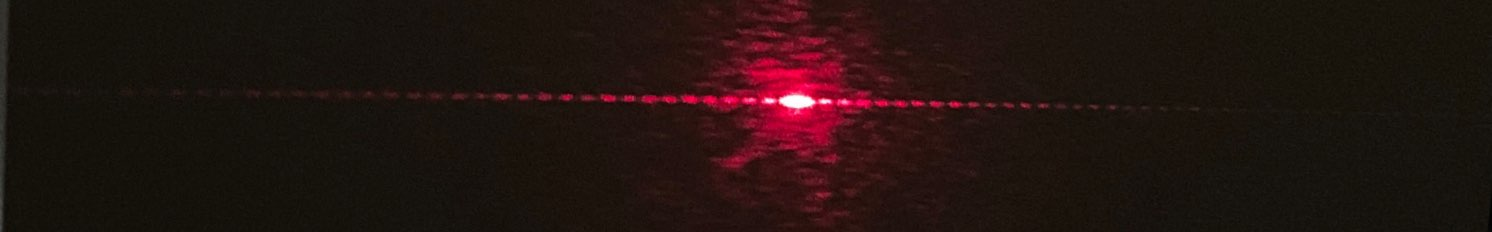
\includegraphics[width=\columnwidth]{assets/4 衍射实验/狭缝 3.jpg}
    \caption{单缝 3 (宽 0.3 mm)}
\end{subfigure}
\caption{单缝衍射现象}
\end{figure}

\begin{figure}[H]\centering
    \begin{subfigure}[b]{\columnwidth}\centering
        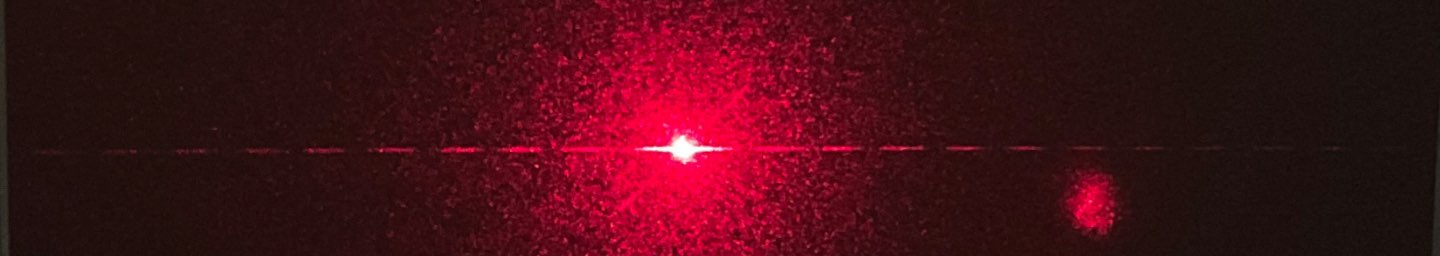
\includegraphics[width=\columnwidth]{assets/4 衍射实验/细条 1.jpg}
        \caption{单丝 1 (宽 0.1 mm)}
    \end{subfigure}\hfill
    \begin{subfigure}[b]{\columnwidth}\centering
        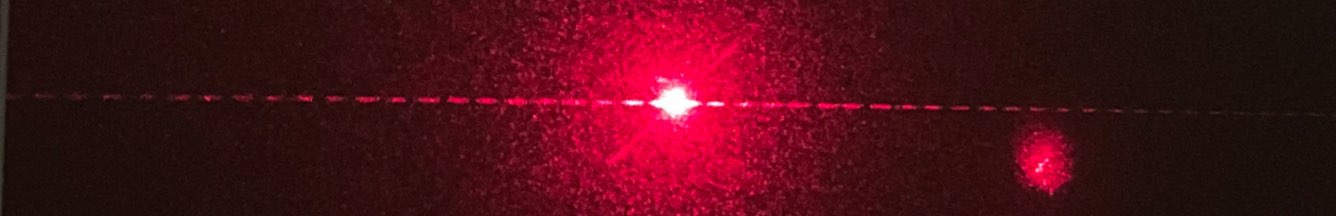
\includegraphics[width=\columnwidth]{assets/4 衍射实验/细条 2.jpg}
        \caption{单丝 2 (宽 0.2 mm)}
    \end{subfigure}
    \begin{subfigure}[b]{\columnwidth}\centering
        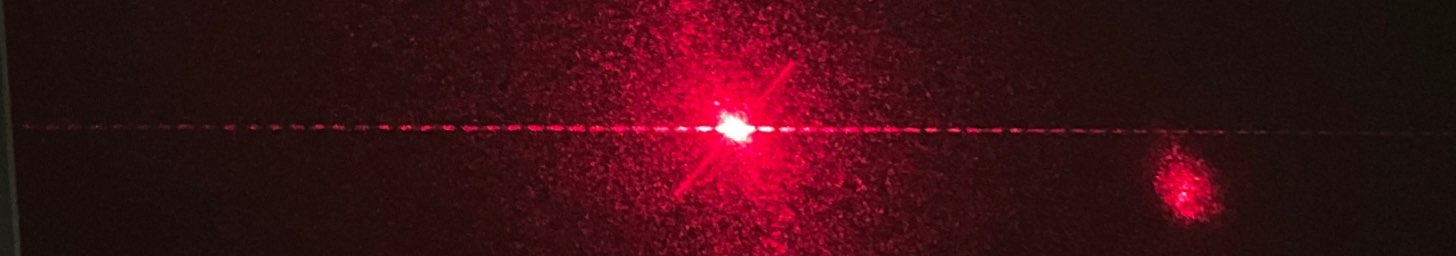
\includegraphics[width=\columnwidth]{assets/4 衍射实验/细条 3.jpg}
        \caption{单丝 3 (宽 0.3 mm)}
    \end{subfigure}
\caption{单丝衍射现象}
\end{figure}

\begin{figure}[H]\centering
\begin{subfigure}[b]{0.33\columnwidth}\centering
    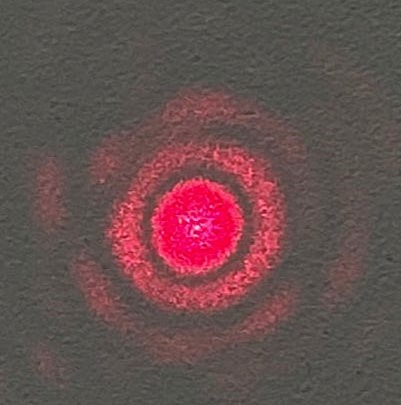
\includegraphics[height=120pt]{assets/4 衍射实验/小孔 1.jpg}
    \caption{小孔 1 (直径 0.2 mm)}
\end{subfigure}\hfill
\begin{subfigure}[b]{0.33\columnwidth}\centering
    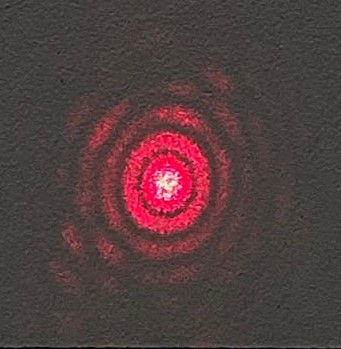
\includegraphics[height=120pt]{assets/4 衍射实验/小孔 2.jpg}
    \caption{小孔 2 (直径 0.3 mm)}
\end{subfigure}
\begin{subfigure}[b]{0.33\columnwidth}\centering
    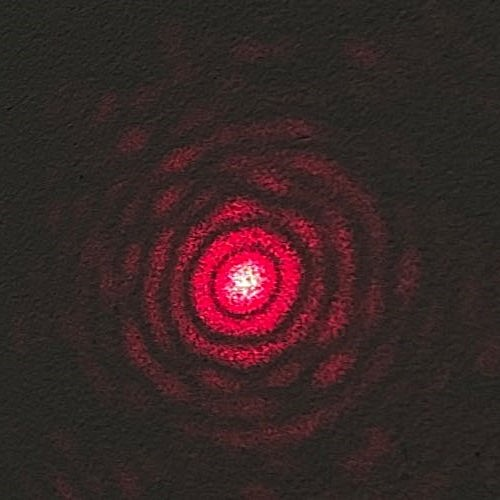
\includegraphics[height=120pt]{assets/4 衍射实验/小孔 3.jpg}
    \caption{小孔 3 (直径 0.4 mm)}
\end{subfigure}
\caption{小孔衍射现象}
\end{figure}

\begin{figure}[H]\centering
    
\includegraphics[width=0.7\columnwidth]{assets/4 衍射实验/圆点.jpg}
    \caption{小屏时观察不到衍射现象}\label{小孔衍射现象}
\end{figure}

\subsubsection{光谱仪测光谱}

该实验光路中只有待测光源、光谱仪接收器两个部分,后者与支架连接固定,将光谱仪连接到电脑,打开电脑的 SpectraSmart 软件,就可以看到光谱图像。我们依次测量了白光 LED、红色半导体激光和手机手电筒的光谱数据,如下所示。

\begin{figure}[H]\centering
    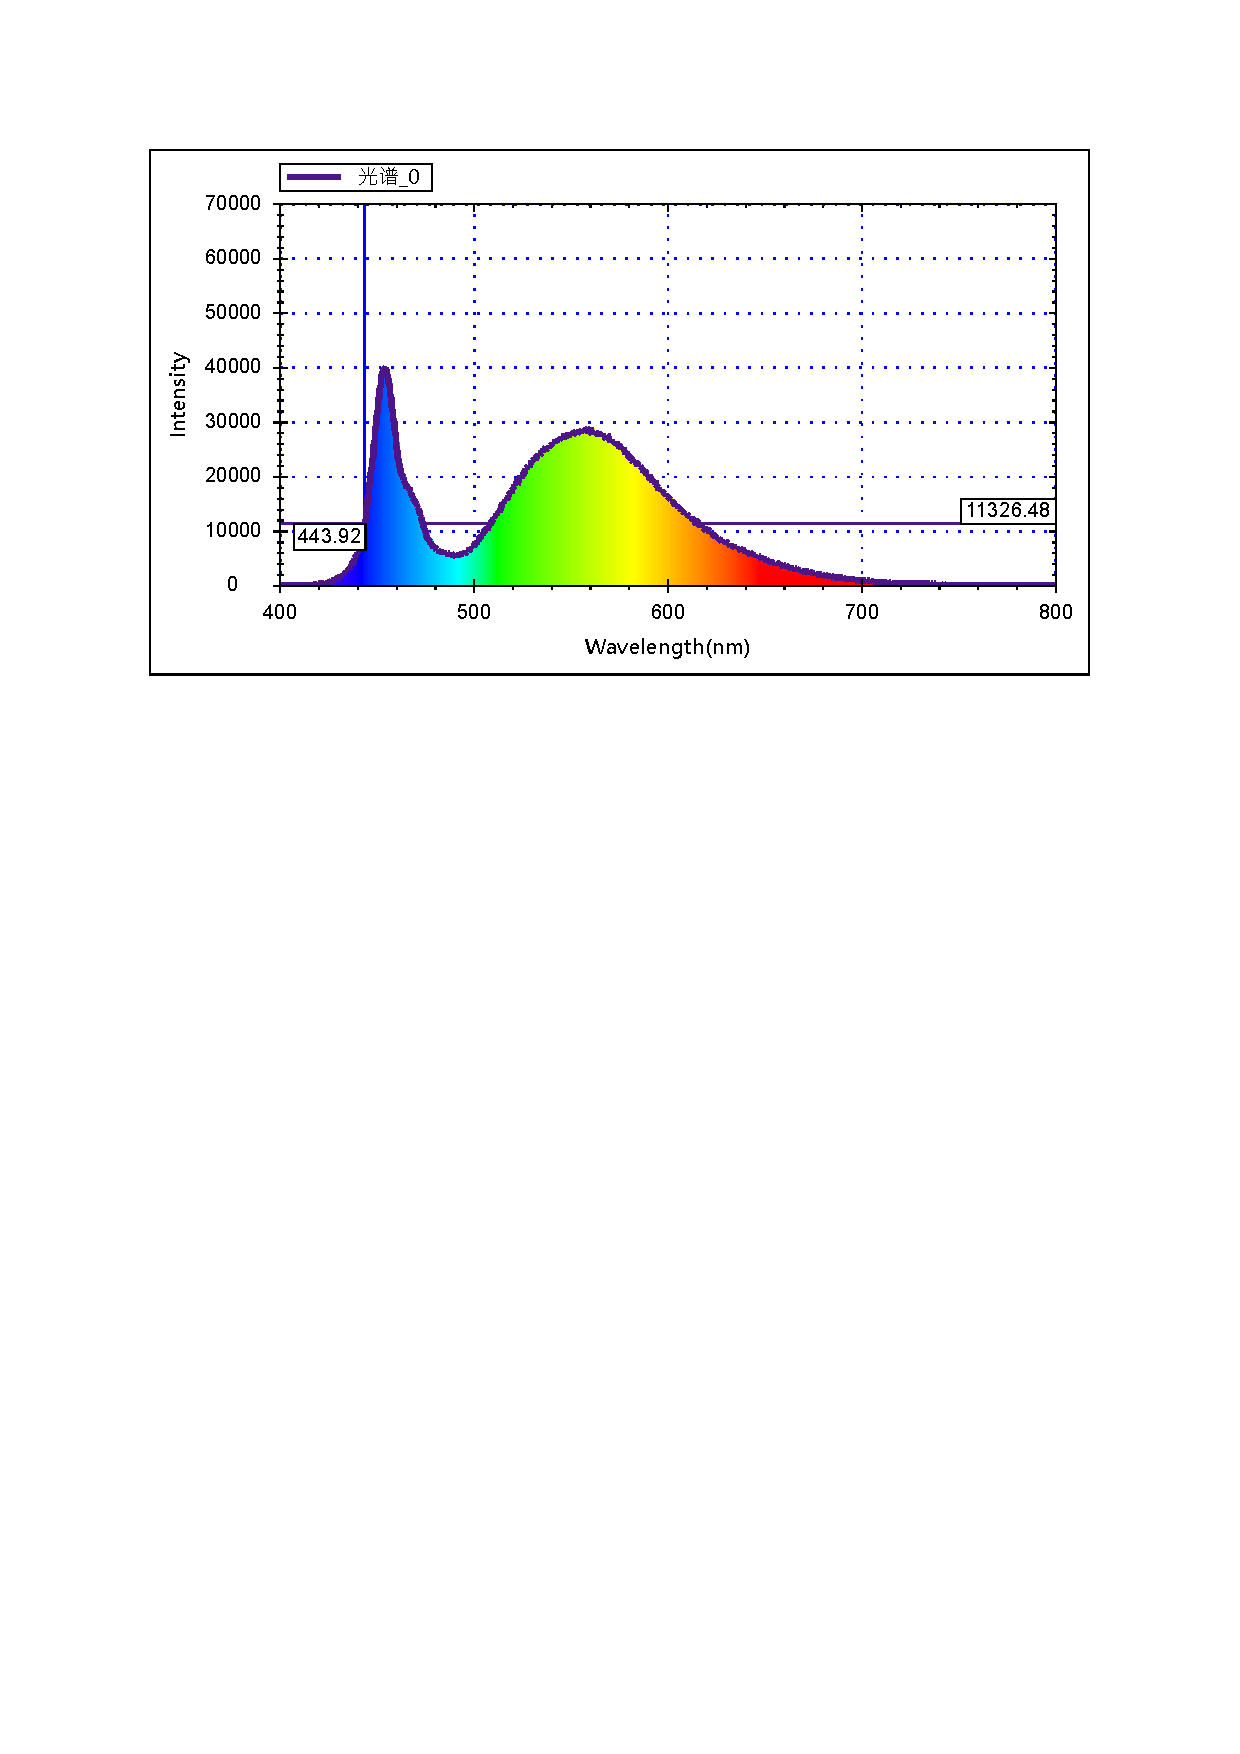
\includegraphics[width=\columnwidth]{assets/5 光谱仪/白光 LED.pdf}
    \caption{白光 LED 光谱测量结果}
\end{figure}
\begin{figure}[H]\centering
    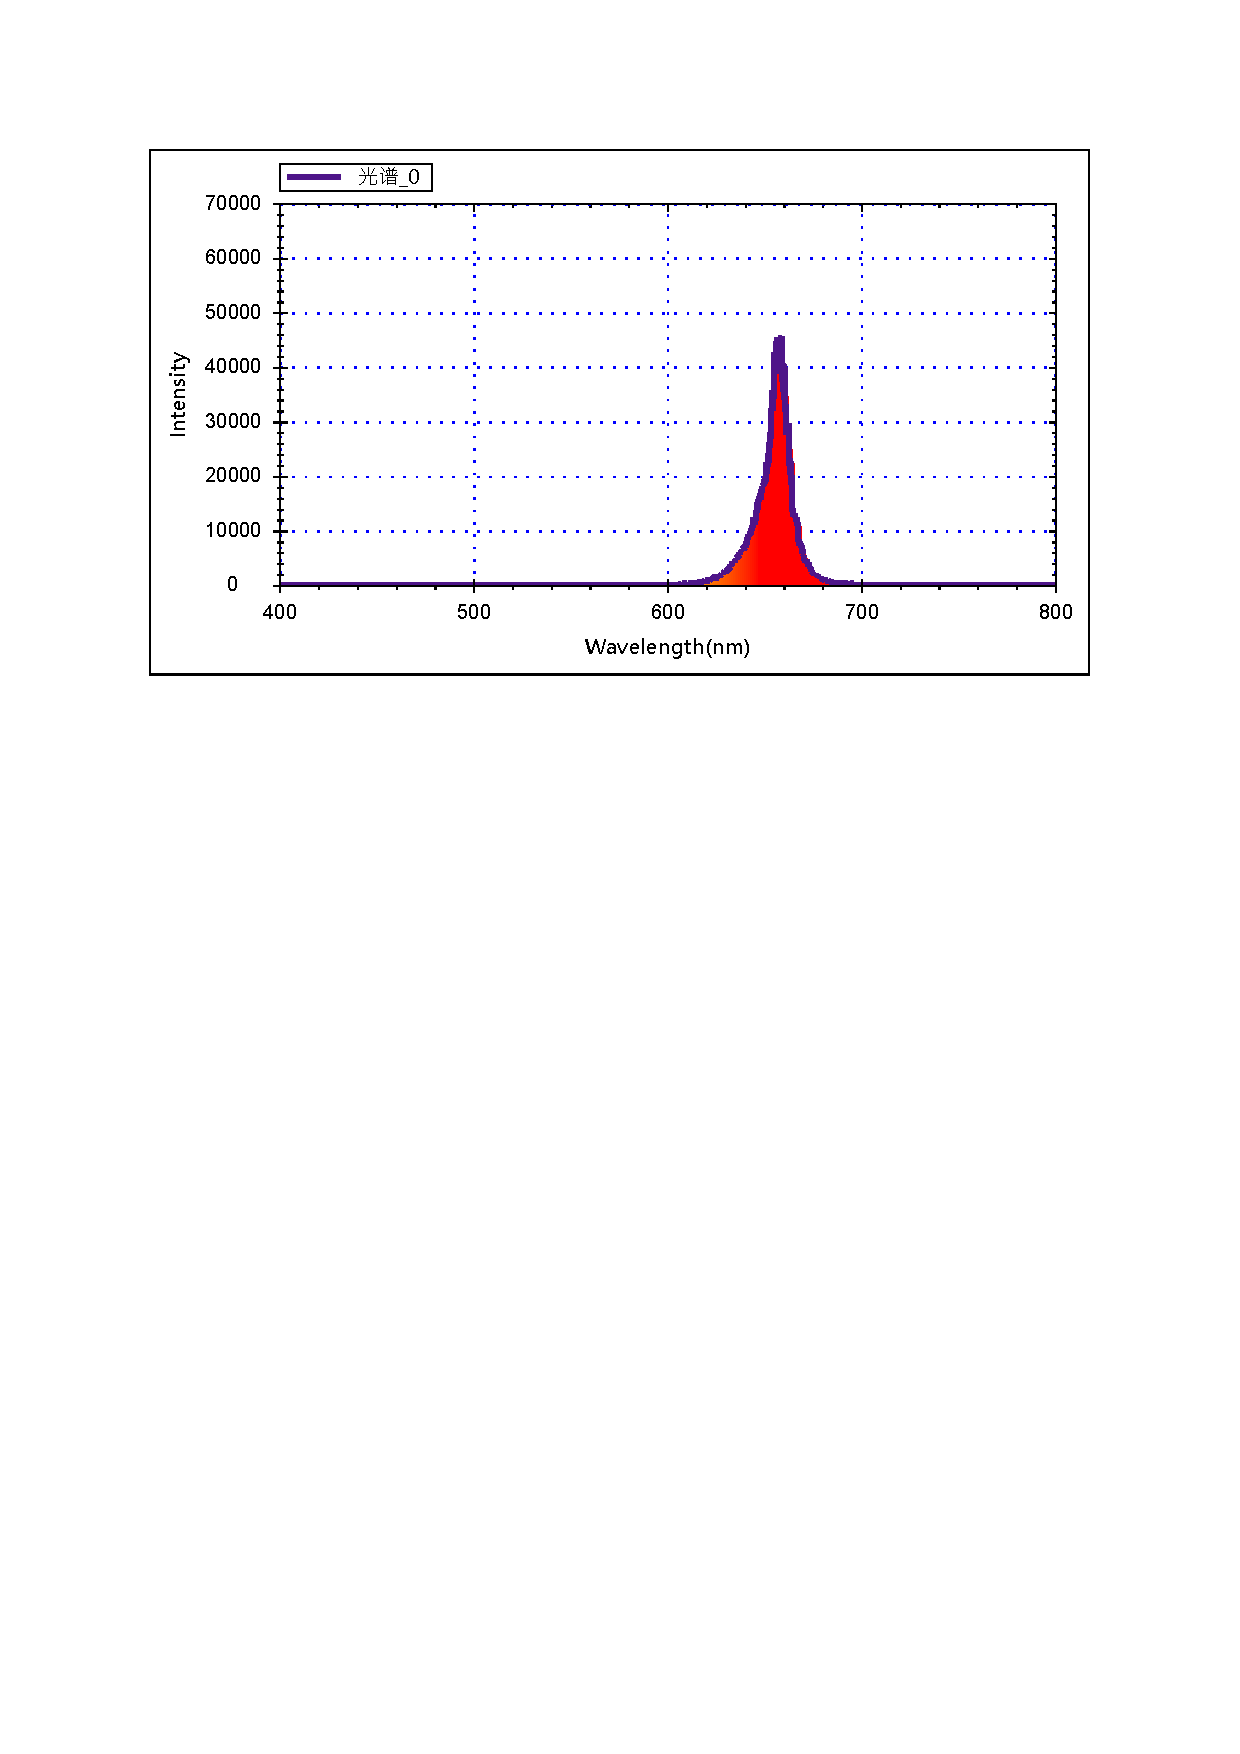
\includegraphics[width=\columnwidth]{assets/5 光谱仪/红光激光.pdf}
    \caption{白光 LED 光谱测量结果}
\end{figure}
\begin{figure}[H]\centering
    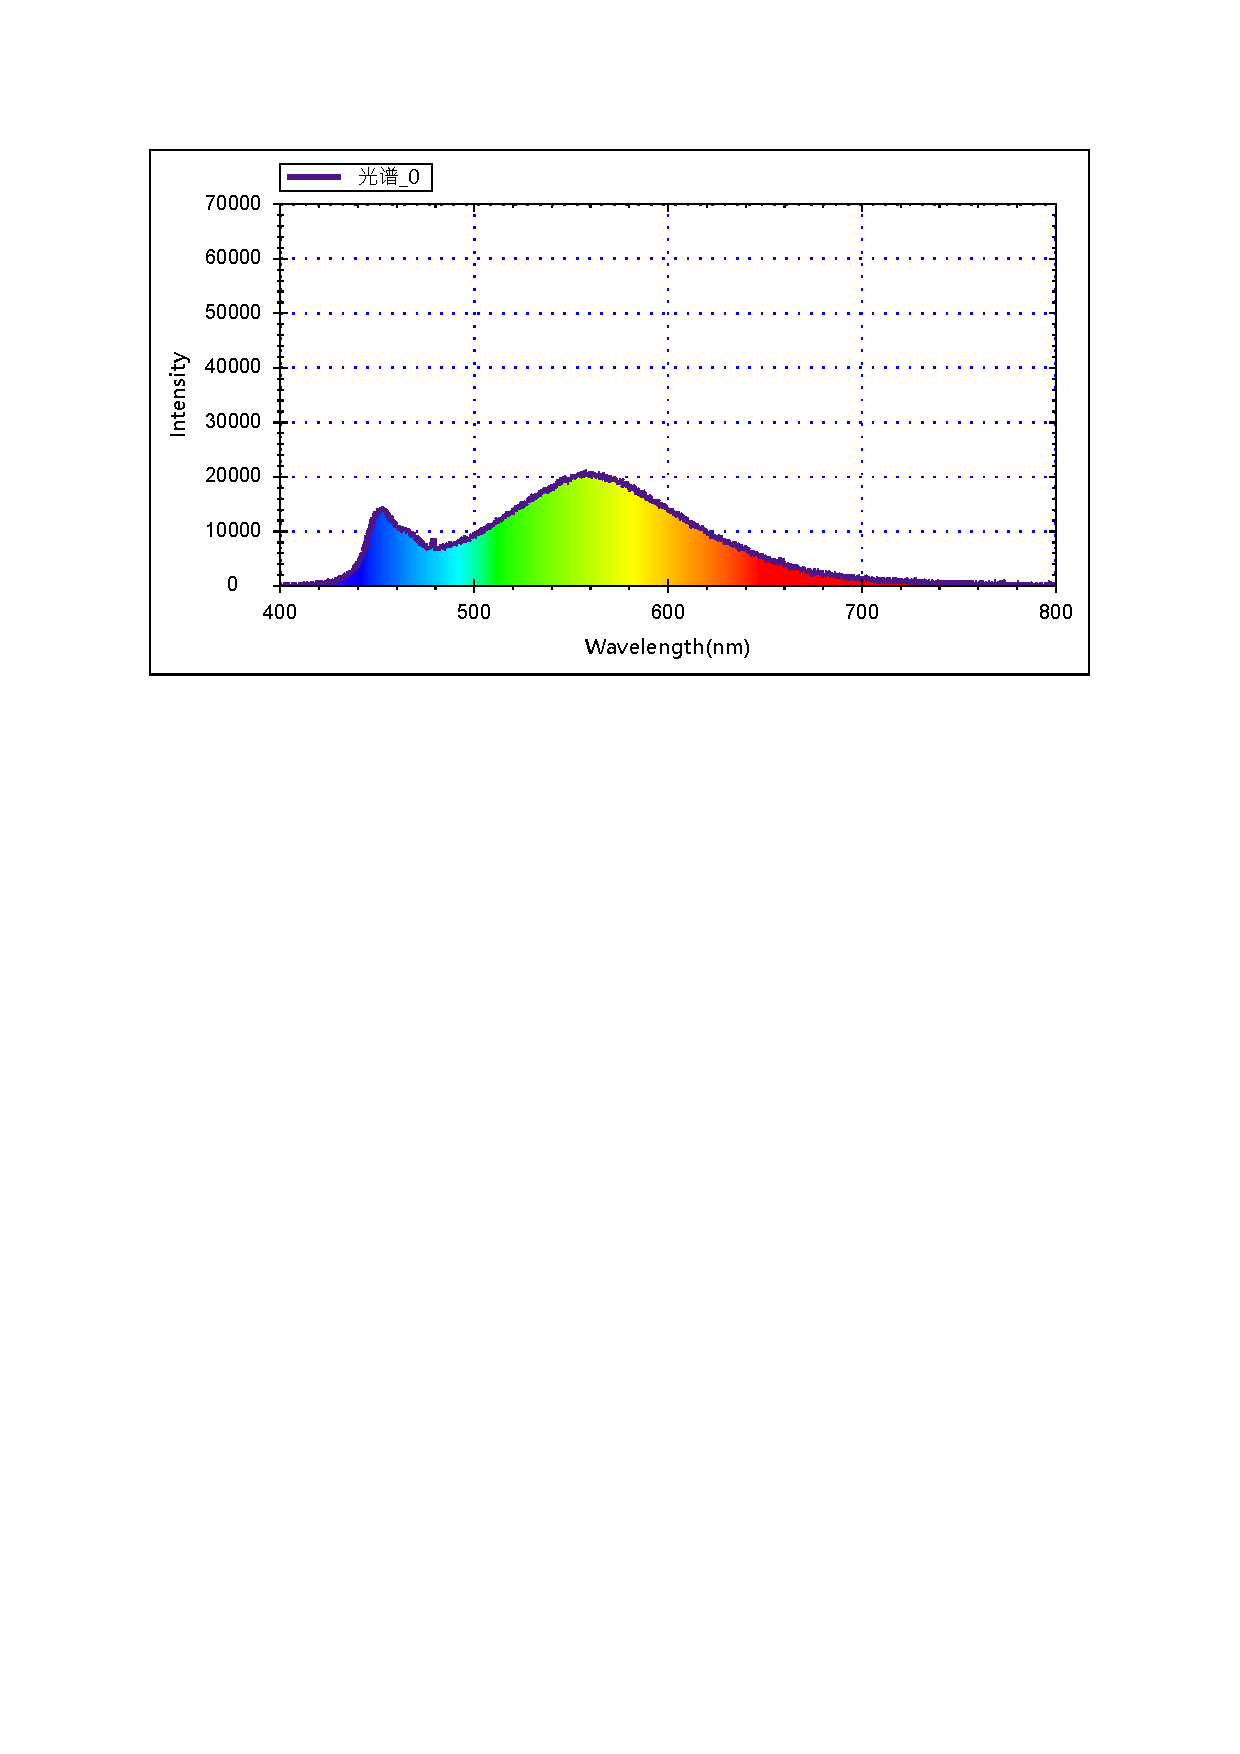
\includegraphics[width=\columnwidth]{assets/5 光谱仪/手机手电筒.pdf}
    \caption{白光 LED 光谱测量结果}
\end{figure}

从图中我们可以看出,实际中的单色光(即使是激光)都不是由纯粹单一波长的光所构成,而是由一个波长范围里的光复合而得,这些颜色加强了该光的颜色(或被该光颜色波段较强的光掩盖),或者由多种光复合而成,从而只显现出一种颜色。

导出各光谱的数据,到 Matlab 中作出精确图像,如下所示:

\begin{figure}[H]\centering
    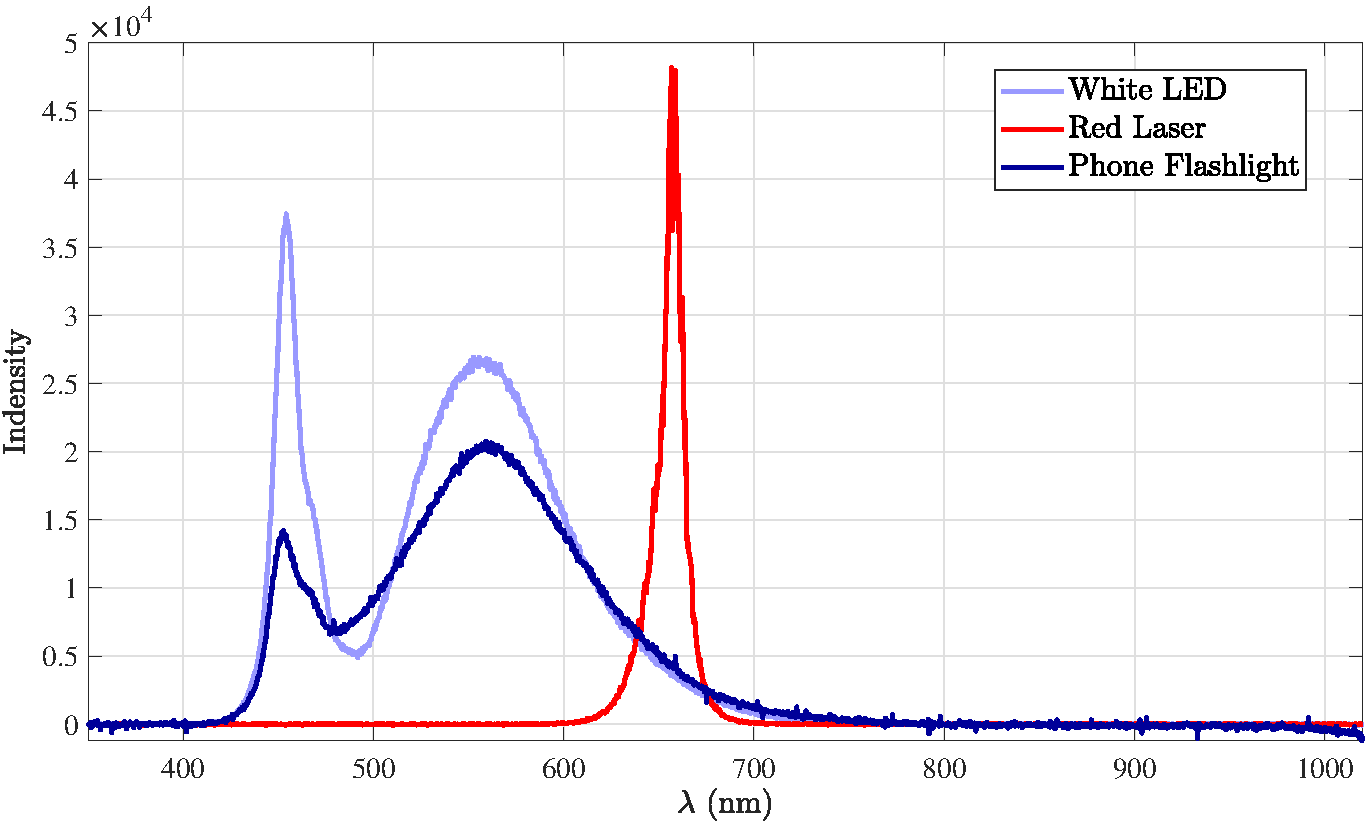
\includegraphics[width=\columnwidth]{assets/5 光谱仪/2024-11-06_00-44-38.pdf}
    \caption{三种光源的光谱结果}\label{三种光源的光谱结果}
\end{figure}

为了得到红色镭射激光的主波长,我们对其光谱数据进行了拟合(采用三重高斯拟合),如图 \ref{红色镭射激光数据拟合效果} 所示,拟合优度相关参数如下:
\begin{equation}
R^2 = 0.9997367,\quad R^2_{\text{adj}} = 0.9997356,\quad \text{SSE} = 1.3620 \times 10^7,\quad \text{RMSE} = 83.5527
\end{equation}
\begin{figure}[H]\centering
    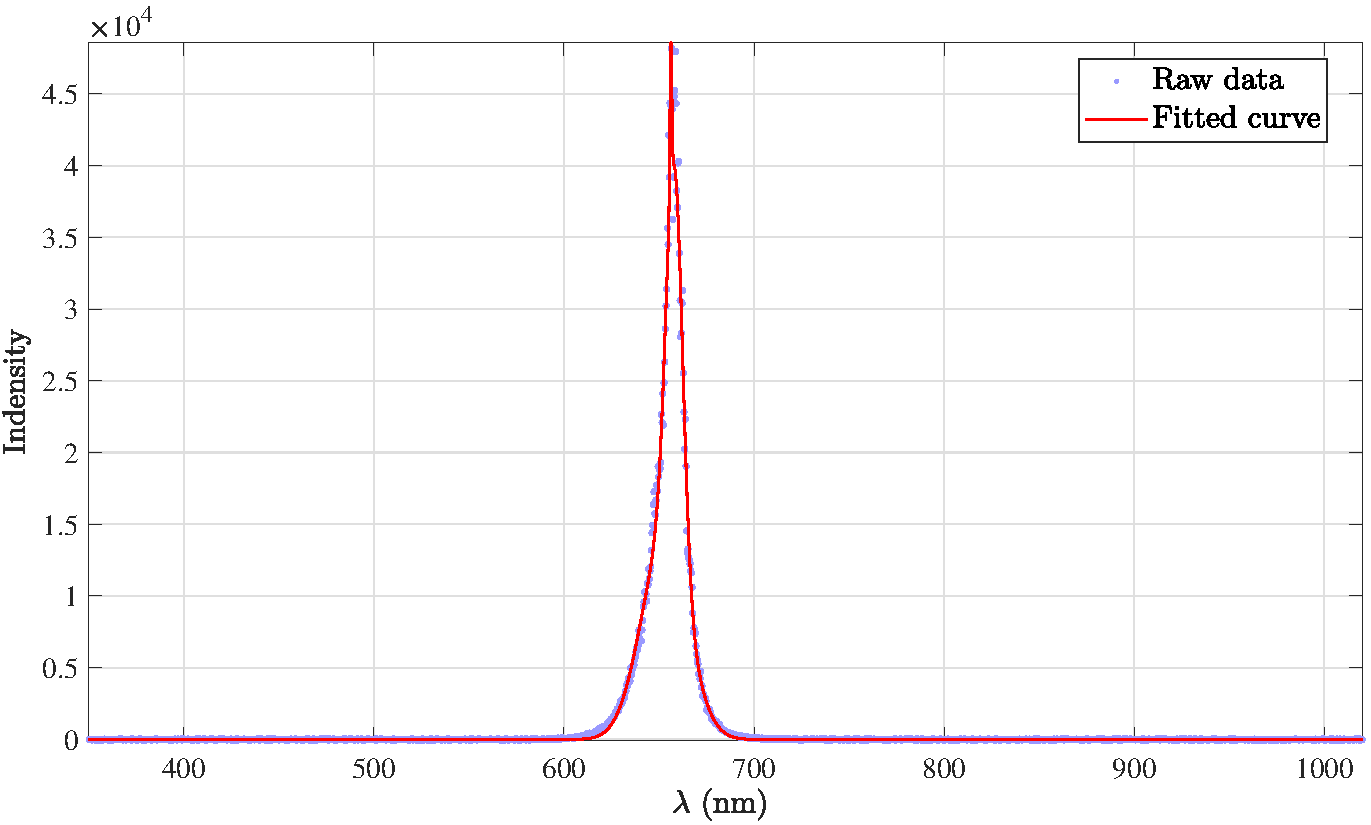
\includegraphics[width=\columnwidth]{assets/5 光谱仪/2024-11-06_00-56-48.pdf}
    \caption{红色镭射激光数据拟合效果}\label{红色镭射激光数据拟合效果}
\end{figure}

\begin{figure}[H]\centering
    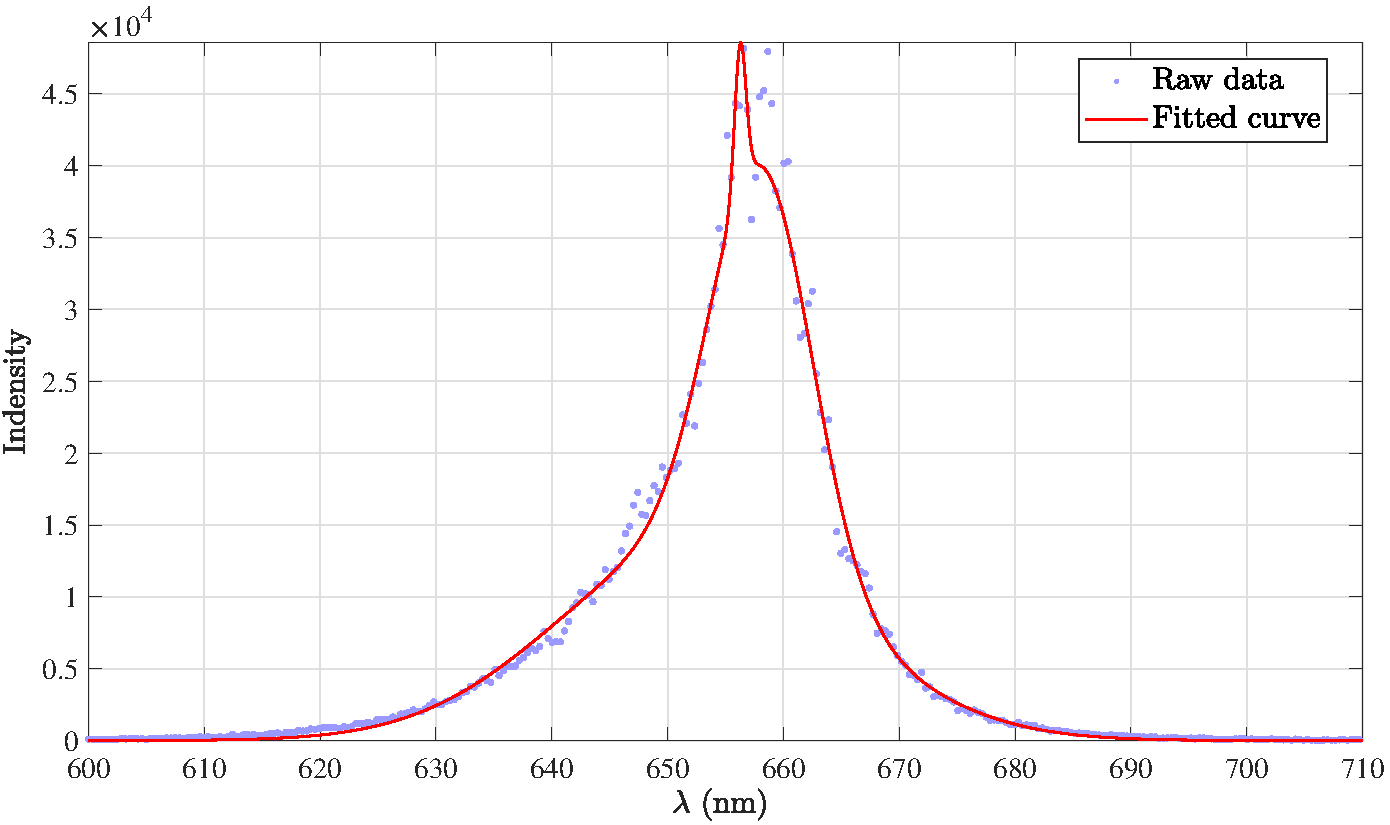
\includegraphics[width=\columnwidth]{assets/5 光谱仪/2024-11-06_01-19-00.pdf}
    \caption{拟合局部放大}\label{拟合局部放大}
\end{figure}


由优度参数与图像可知,拟合效果极好。依据拟合函数,即可求出光强最大点对应的波长值\footnote{Matlab 源码见附录 B} : 
\begin{equation}\boldmath
    \lambda = 656.3226\ \mathrm{nm}
\end{equation}

\subsection{光栅、夫琅禾费衍射与光谱仪测量光谱实验总结}

\begin{graybox}
\textbf{光栅、夫琅禾费衍射与光谱仪测量光谱实验总结:}

本次实验“光栅与光栅仪器”分为三个部分:
一是测量透射光栅的每毫米刻缝数,通过实验得到 $N\approx100$ ,与实际值符合得很好;二是观察夫琅禾费衍射,实验现象明显,但小屏实验无法观察到衍射现象;
三是利用 SpectraSmart 软件观察白光 LED 等不同光源的光谱,我们还对红色镭射激光的光谱数据进行了拟合并以此求解主波长,实验简单而有趣。
\end{graybox}



\section{实验思考题}

\subsection*{5.1 阿贝成像思考题}
\subsubsection*{5.1.1 阿贝成像中,当“缝”与光栅方向夹角 45 度放置滤波时,会有何效果?}
如图 \ref{45 度} 所示,当“缝”与光栅方向夹角 45 度放置滤波时,“光”字像会有斜 45 度条纹。
\begin{figure}[H]\centering
    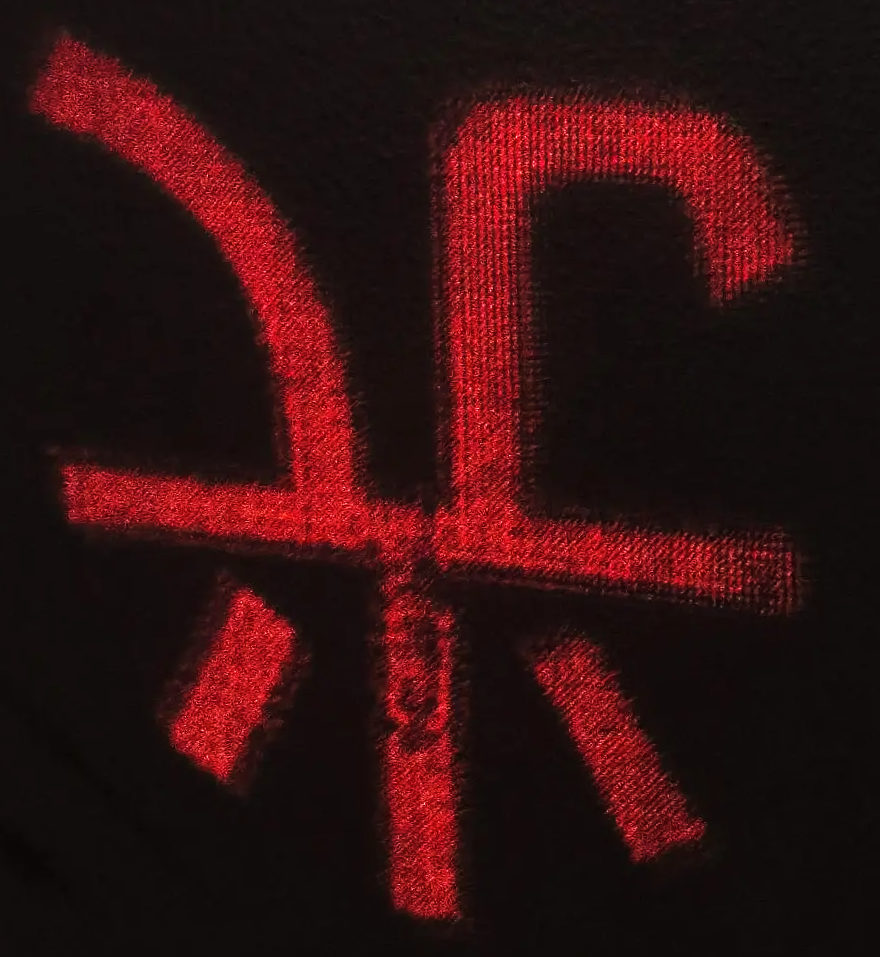
\includegraphics[width=0.5\columnwidth]{assets/1 阿贝尔/光 45度.png}
    \caption{“缝”与光栅方向夹角 45 度}\label{45 度}
\end{figure}

\subsubsection*{5.1.2 前面实验中,我们使用低通滤波(仅让 0 级斑通过)实现了光栅格子信息的消除;如何做个高通滤波的例子?应该如何实现和它的效果是什么?}
裁剪硬纸板,使得 0 级斑及附近光斑被遮挡,而高频光斑未被遮挡,即可实现高通滤波效果,如图 \ref{高通滤波} 所示。

\begin{figure}[H]\centering
\begin{subfigure}[b]{0.5\columnwidth}\centering
    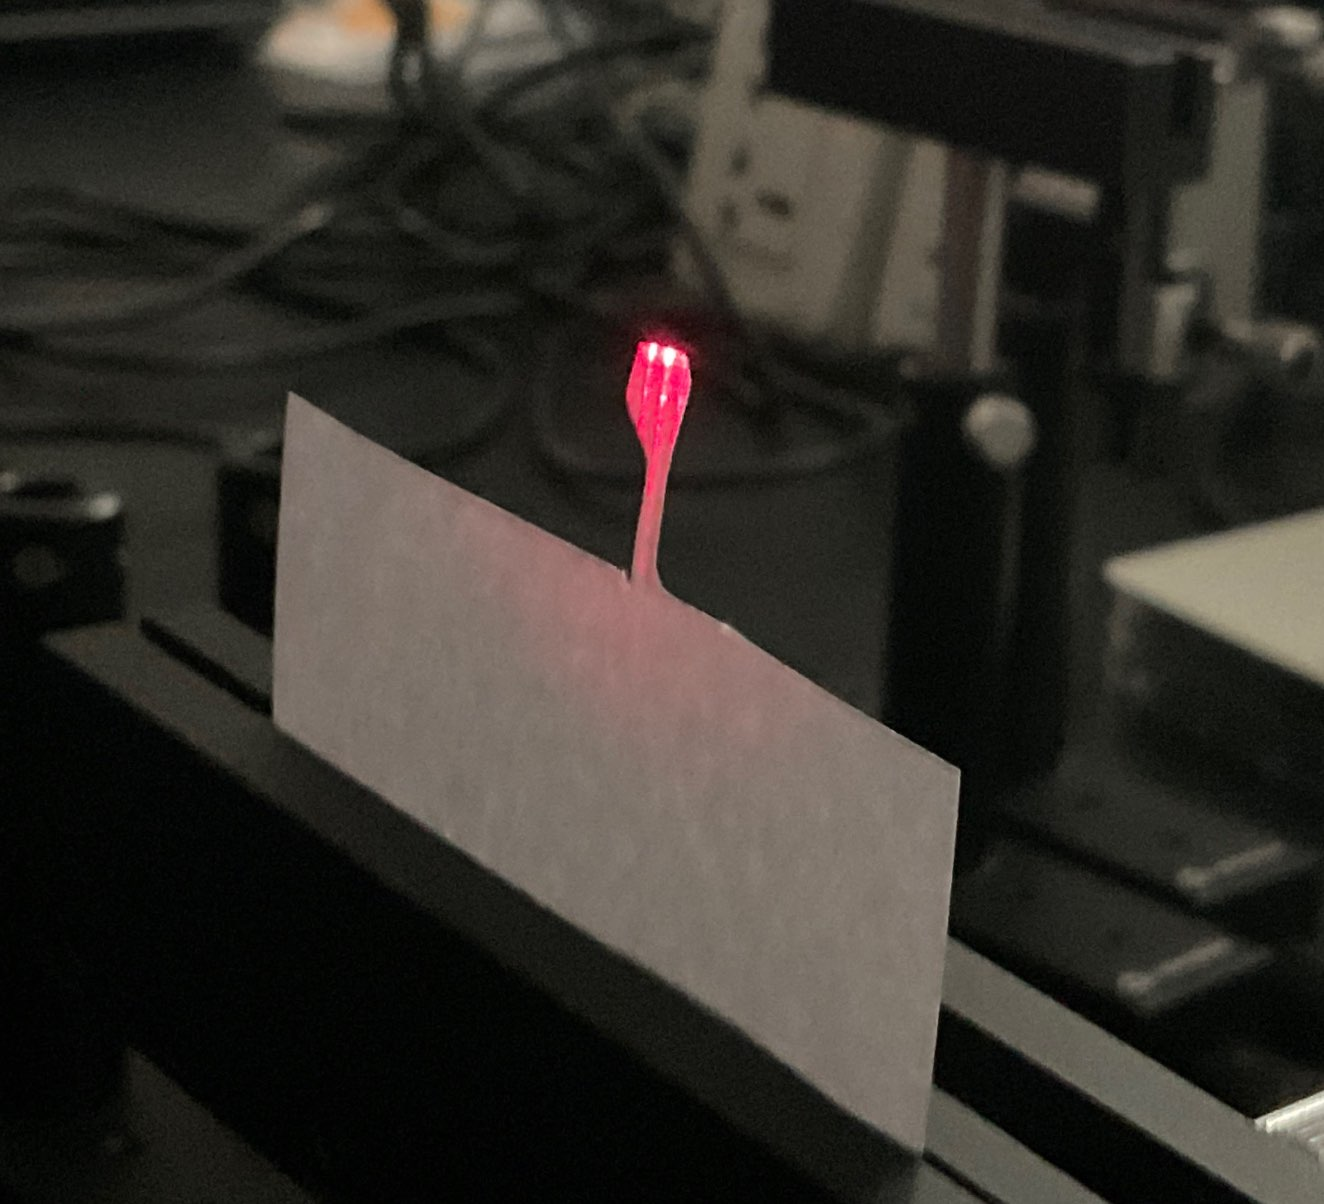
\includegraphics[height=215pt]{assets/1 阿贝尔/自制高通滤波器.jpg}
    \caption{自制高通滤波器}
\end{subfigure}\hfill
\begin{subfigure}[b]{0.5\columnwidth}\centering
    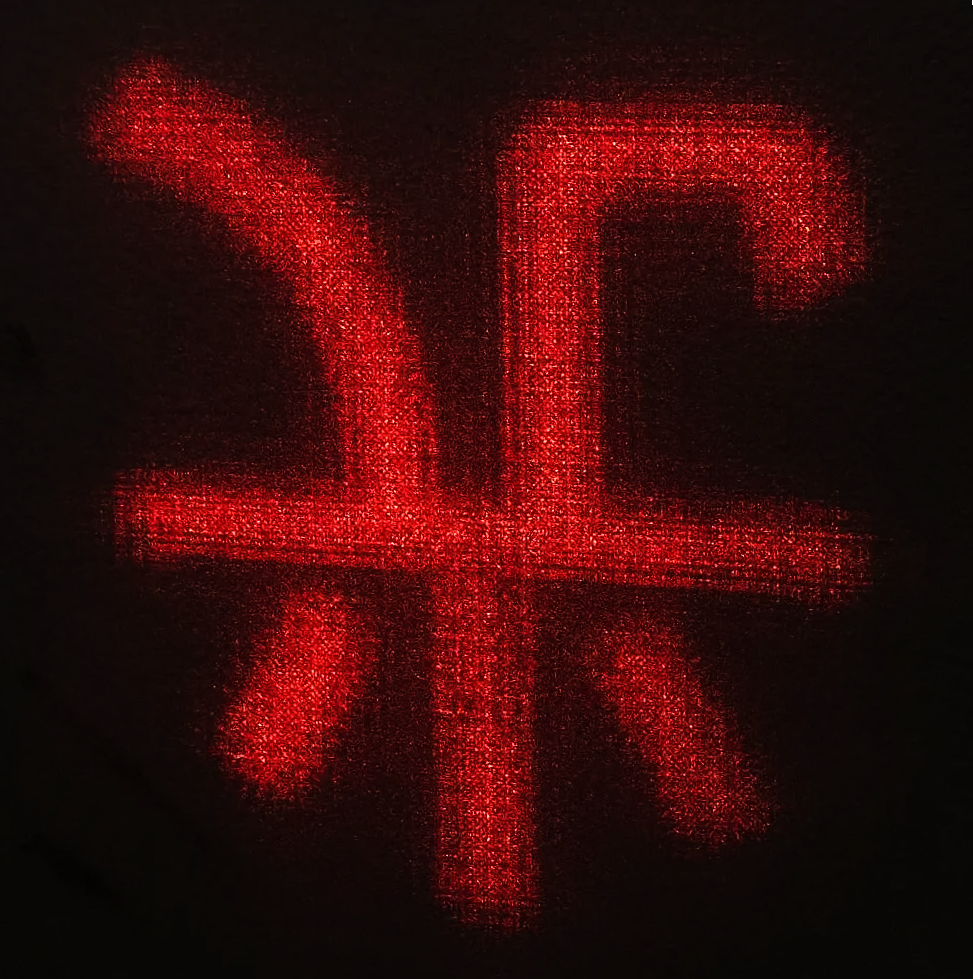
\includegraphics[height=215pt]{assets/1 阿贝尔/光 高通.png}
    \caption{“光”字像}
\end{subfigure}
\caption{高通滤波}\label{高通滤波}
\end{figure}


\subsection*{5.2 观察 4F 系统成像与阿贝成像时单透镜成像的区别是什么?}
与阿贝成像系统相比,4F 系统在白屏上的像清晰且明显,激光透过白纸黑字也能够在白
屏上呈现清晰的像,说明4F 系统保留调制物原有信息的能力更强。


\subsection*{5.3 假彩色编码实验中使用的天安门城楼光栅本身中的城楼的窗户和门洞都是透光的,但是为什么经过所提供的假着色滤波处理后所成的像中这些窗户和门洞是黑色的?有方法验证你的解释吗?}
通过窗户和门洞的光是直接透射,该部分信息聚集在频谱面中心(或者认为通过窗户和门洞的光通过的并非偏振的滤波,而是在各个方向上均有振动),而滤波器中心处没有开孔,所以频谱面中心所传递的图像信息,不能透过滤波器继续传播,白屏上的对应位置就是黑色的。因此,解决方法就是给中心“开孔”,如图 \ref{中心开孔后的自制滤波器} 所示:
\begin{figure}[H]\centering
\begin{subfigure}[b]{0.66\columnwidth}\centering
    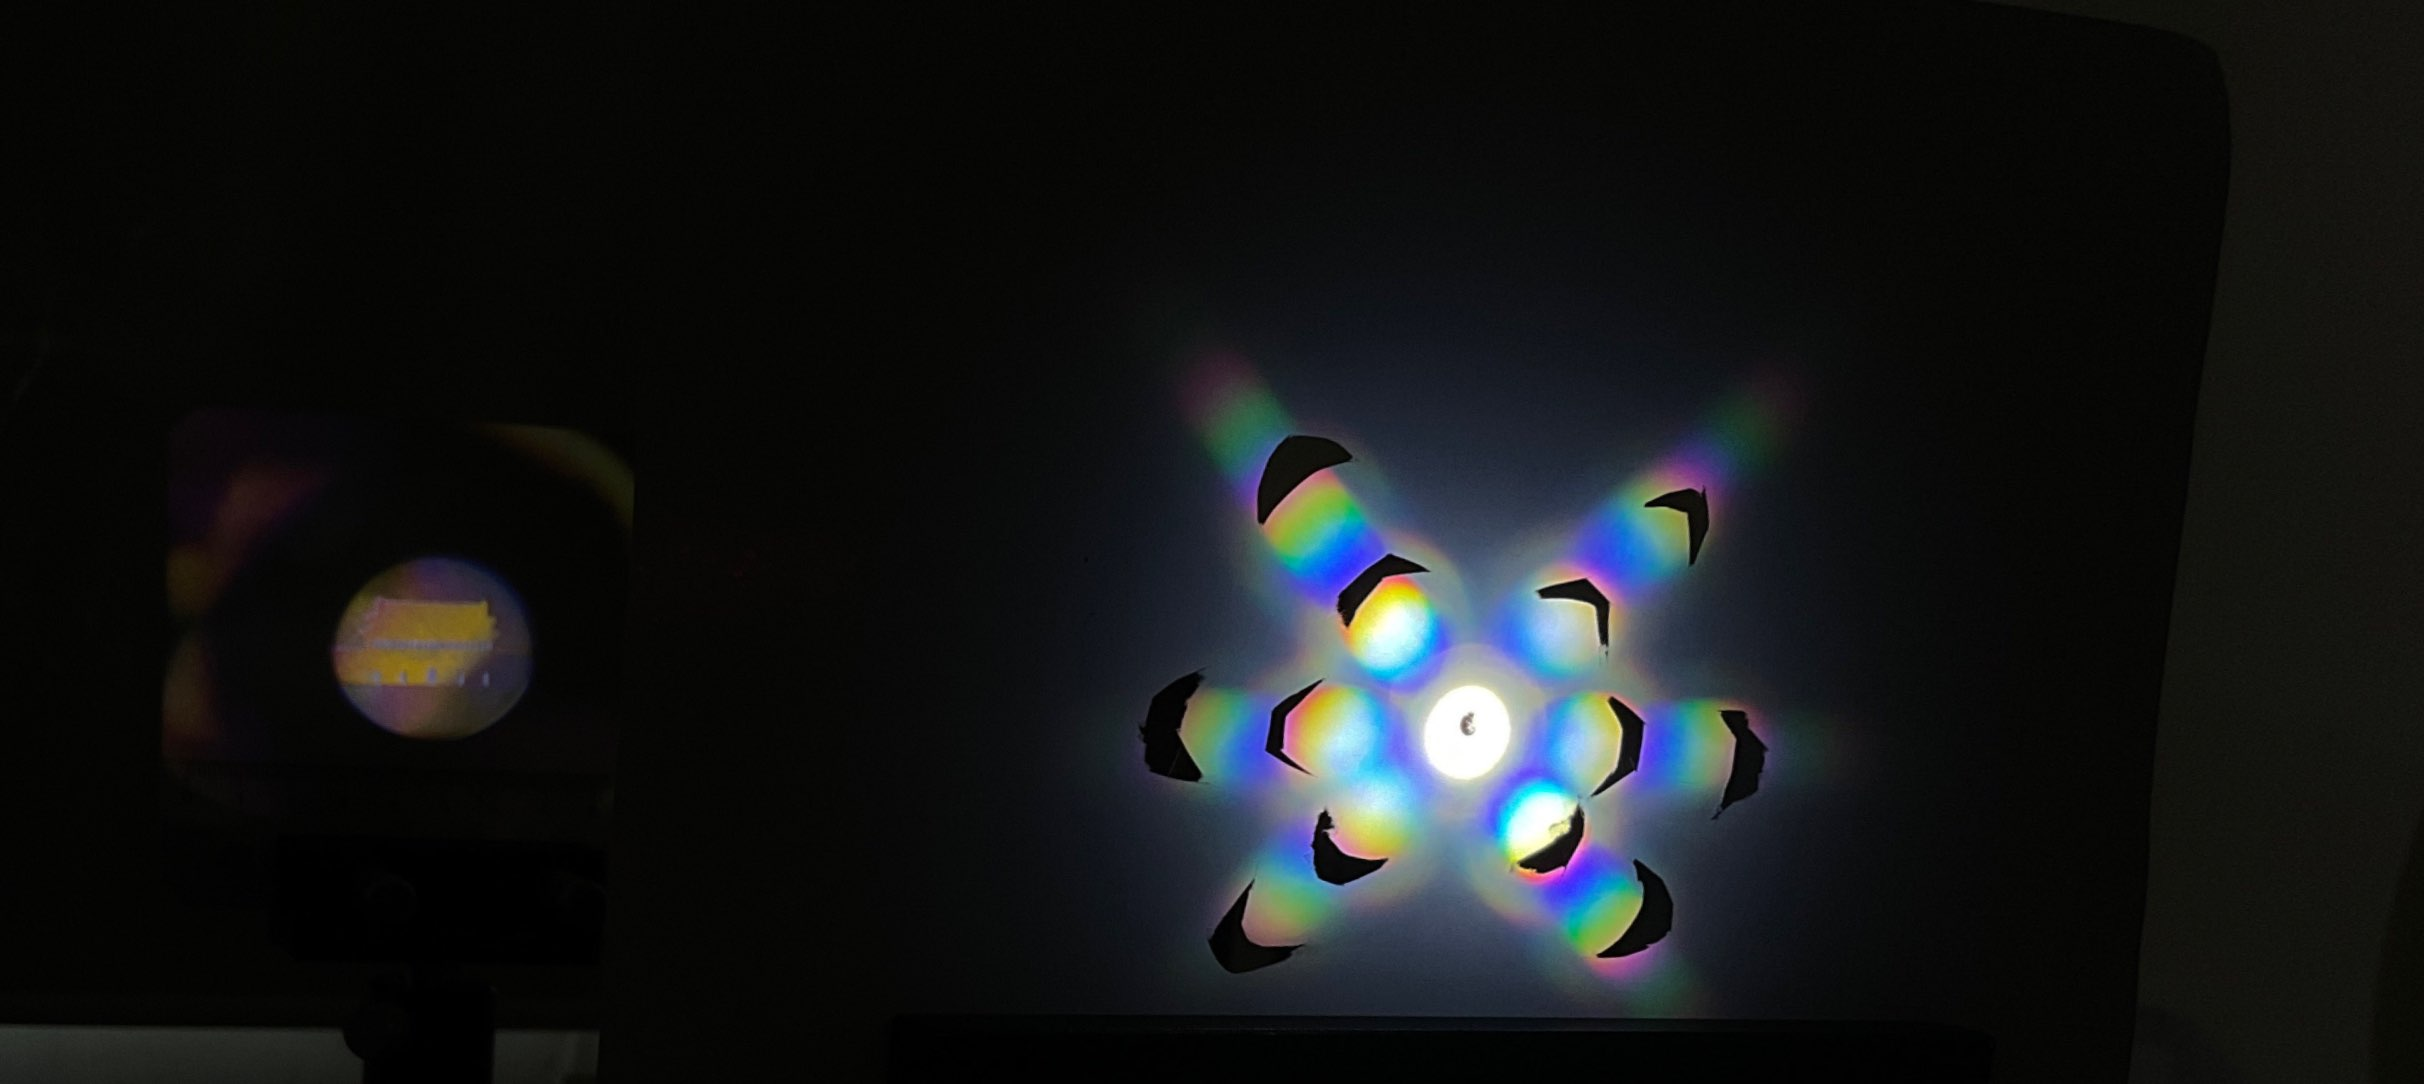
\includegraphics[height=130pt]{assets/3 假彩编码/自制滤波器 亮.jpg}
    \caption{实验台示意图}
\end{subfigure}\hfill
\begin{subfigure}[b]{0.33\columnwidth}\centering
    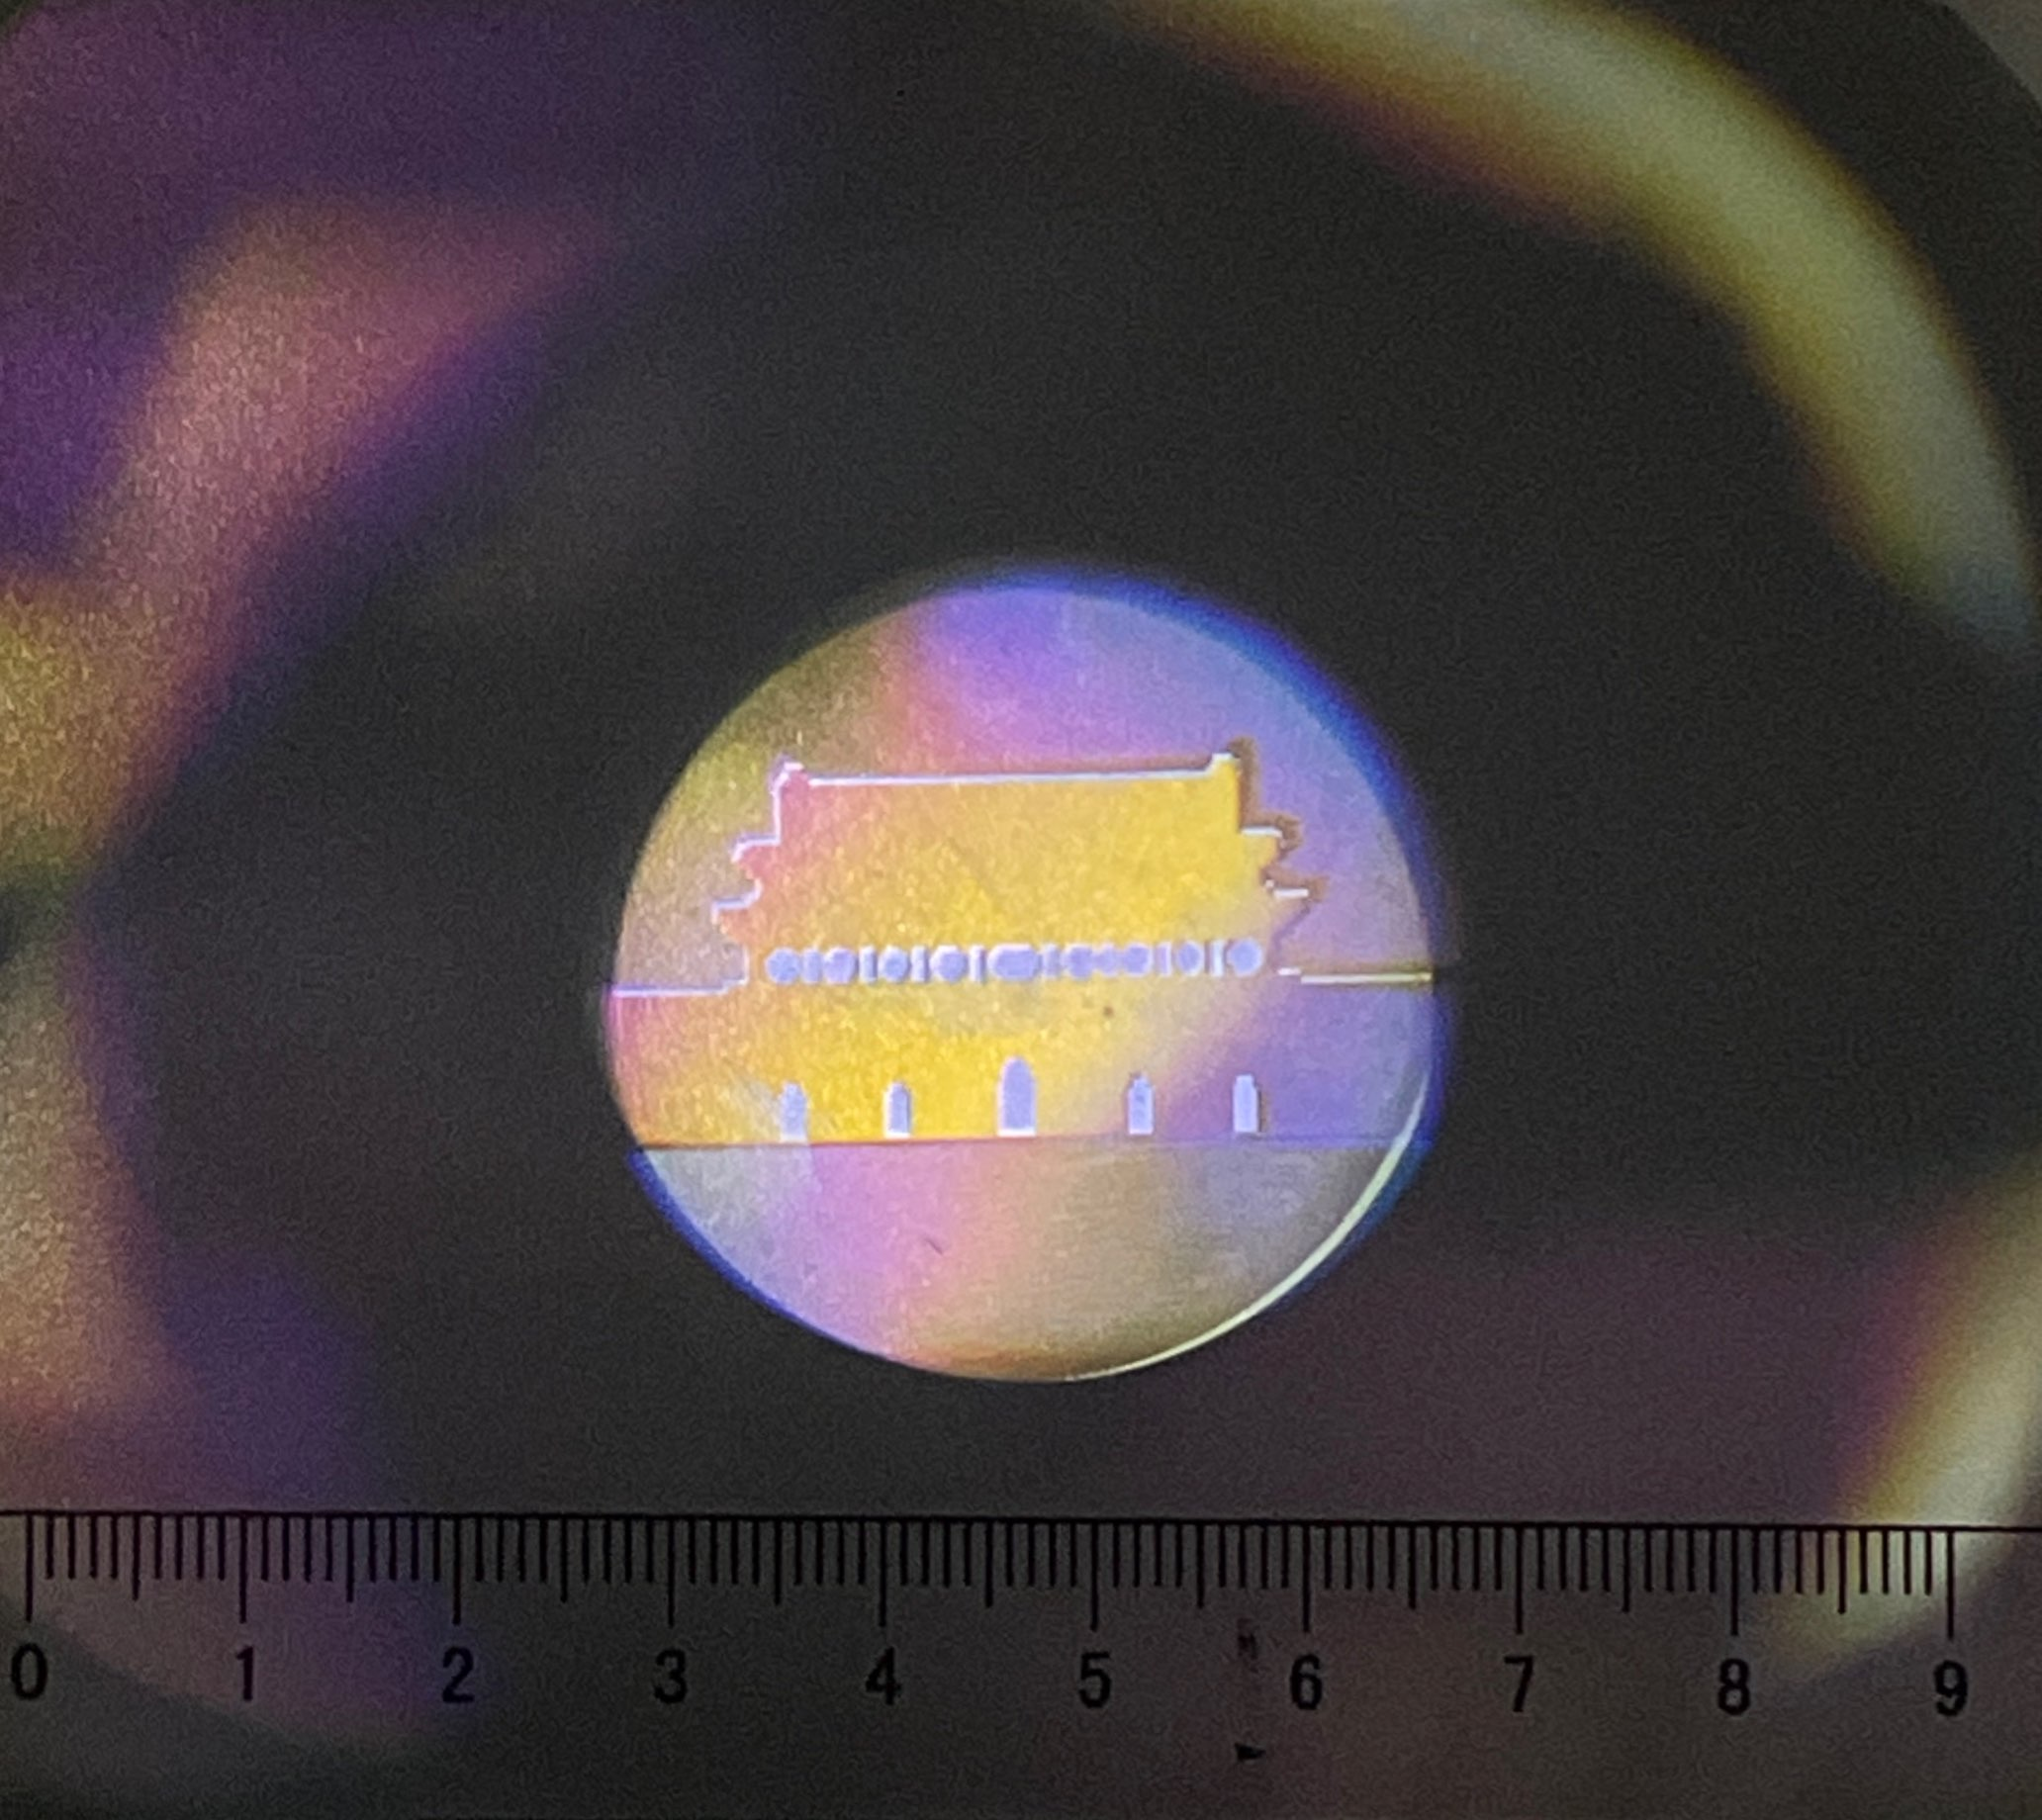
\includegraphics[height=130pt]{assets/3 假彩编码/天安门 自制 亮.jpg}
    \caption{窗户和门洞呈白色的天安门}
\end{subfigure}
\caption{中心开孔后的自制滤波器}
\label{中心开孔后的自制滤波器}
\end{figure}

\subsection*{5.4 从夫琅和费衍射实验得到哪些规律?}
障碍物(屏或丝)或小孔(孔或缝)的尺度越小,衍射现象越明显,但相应的亮度也会减弱。

\section{实验总结与心得体会}

相比于其它实验,此次实验是十分特别地:基本没有数据处理与分析,而是要对实验原理有非常透彻的理解,并依此描述实验所得的图像,解释现象及误差原因,深入浅出。几个子实验都是光学中非常经典的实验,我们在课本上已经或多或少的接触过它们(仅有布拉格衍射还未学过),当我们动手去做这些实验时,才能真正体会到它们的魅力。

实验总体上是成功的,几乎每个小节的实验都与理论符合得较好,所得实验图像也十分具有说服力。

特别地,本次实验我利用 Matlab 软件对最后的光谱实验数据作了进一步的处理和分析,包括换算、拟合、可视化等,相比于常规数据处理和画图方法,这大大提高了分析的准确性和图像的美观性。在今后的实验和研究工作中,我还会继续深入学习和应用类似地计算软件,增强自己的科学计算能力。科研不是考试,我们应该充分利用好自己能接触到的资源,合理使用工具,更高效地发展自身。

另外,这次实验让我感受到,实验“结束”并不意味着实验就已经完成,事实上这仅是数据测量的结束。在课后,我们还需要重新整理实验原理和实验步骤,换算、分析和拟合实验数据,作出合适的数据图,解释可能存在的误差等。在根据已有数据求所需结果时,如何才能最大程度地利用已有数据,同时又尽可能地降低二次误差。上面这些内容都需要体现在最终的实验报告中,一点点累加起来,着实花费了我很多精力。

但最后回过头来,我认为一切都是值得的。当处理完毕的结果十分有力地验证了理论值时(例如光栅的刻线密度),当实验图像与理论近乎“完美”地契合时,心中便迸发出无尽的喜悦,也深深感受到物理“理论与实验结合”的魅力。\footnote{手写预习报告和部分 Matlab 源码附在附录中。}


\newpage
\section*{附录 A\hspace*{20pt} 手写预习报告}
\addcontentsline{toc}{section}{附录 A\hspace*{6pt} 手写预习报告} 
\thispagestyle{fancy} 

\begin{figure}[H]\centering
    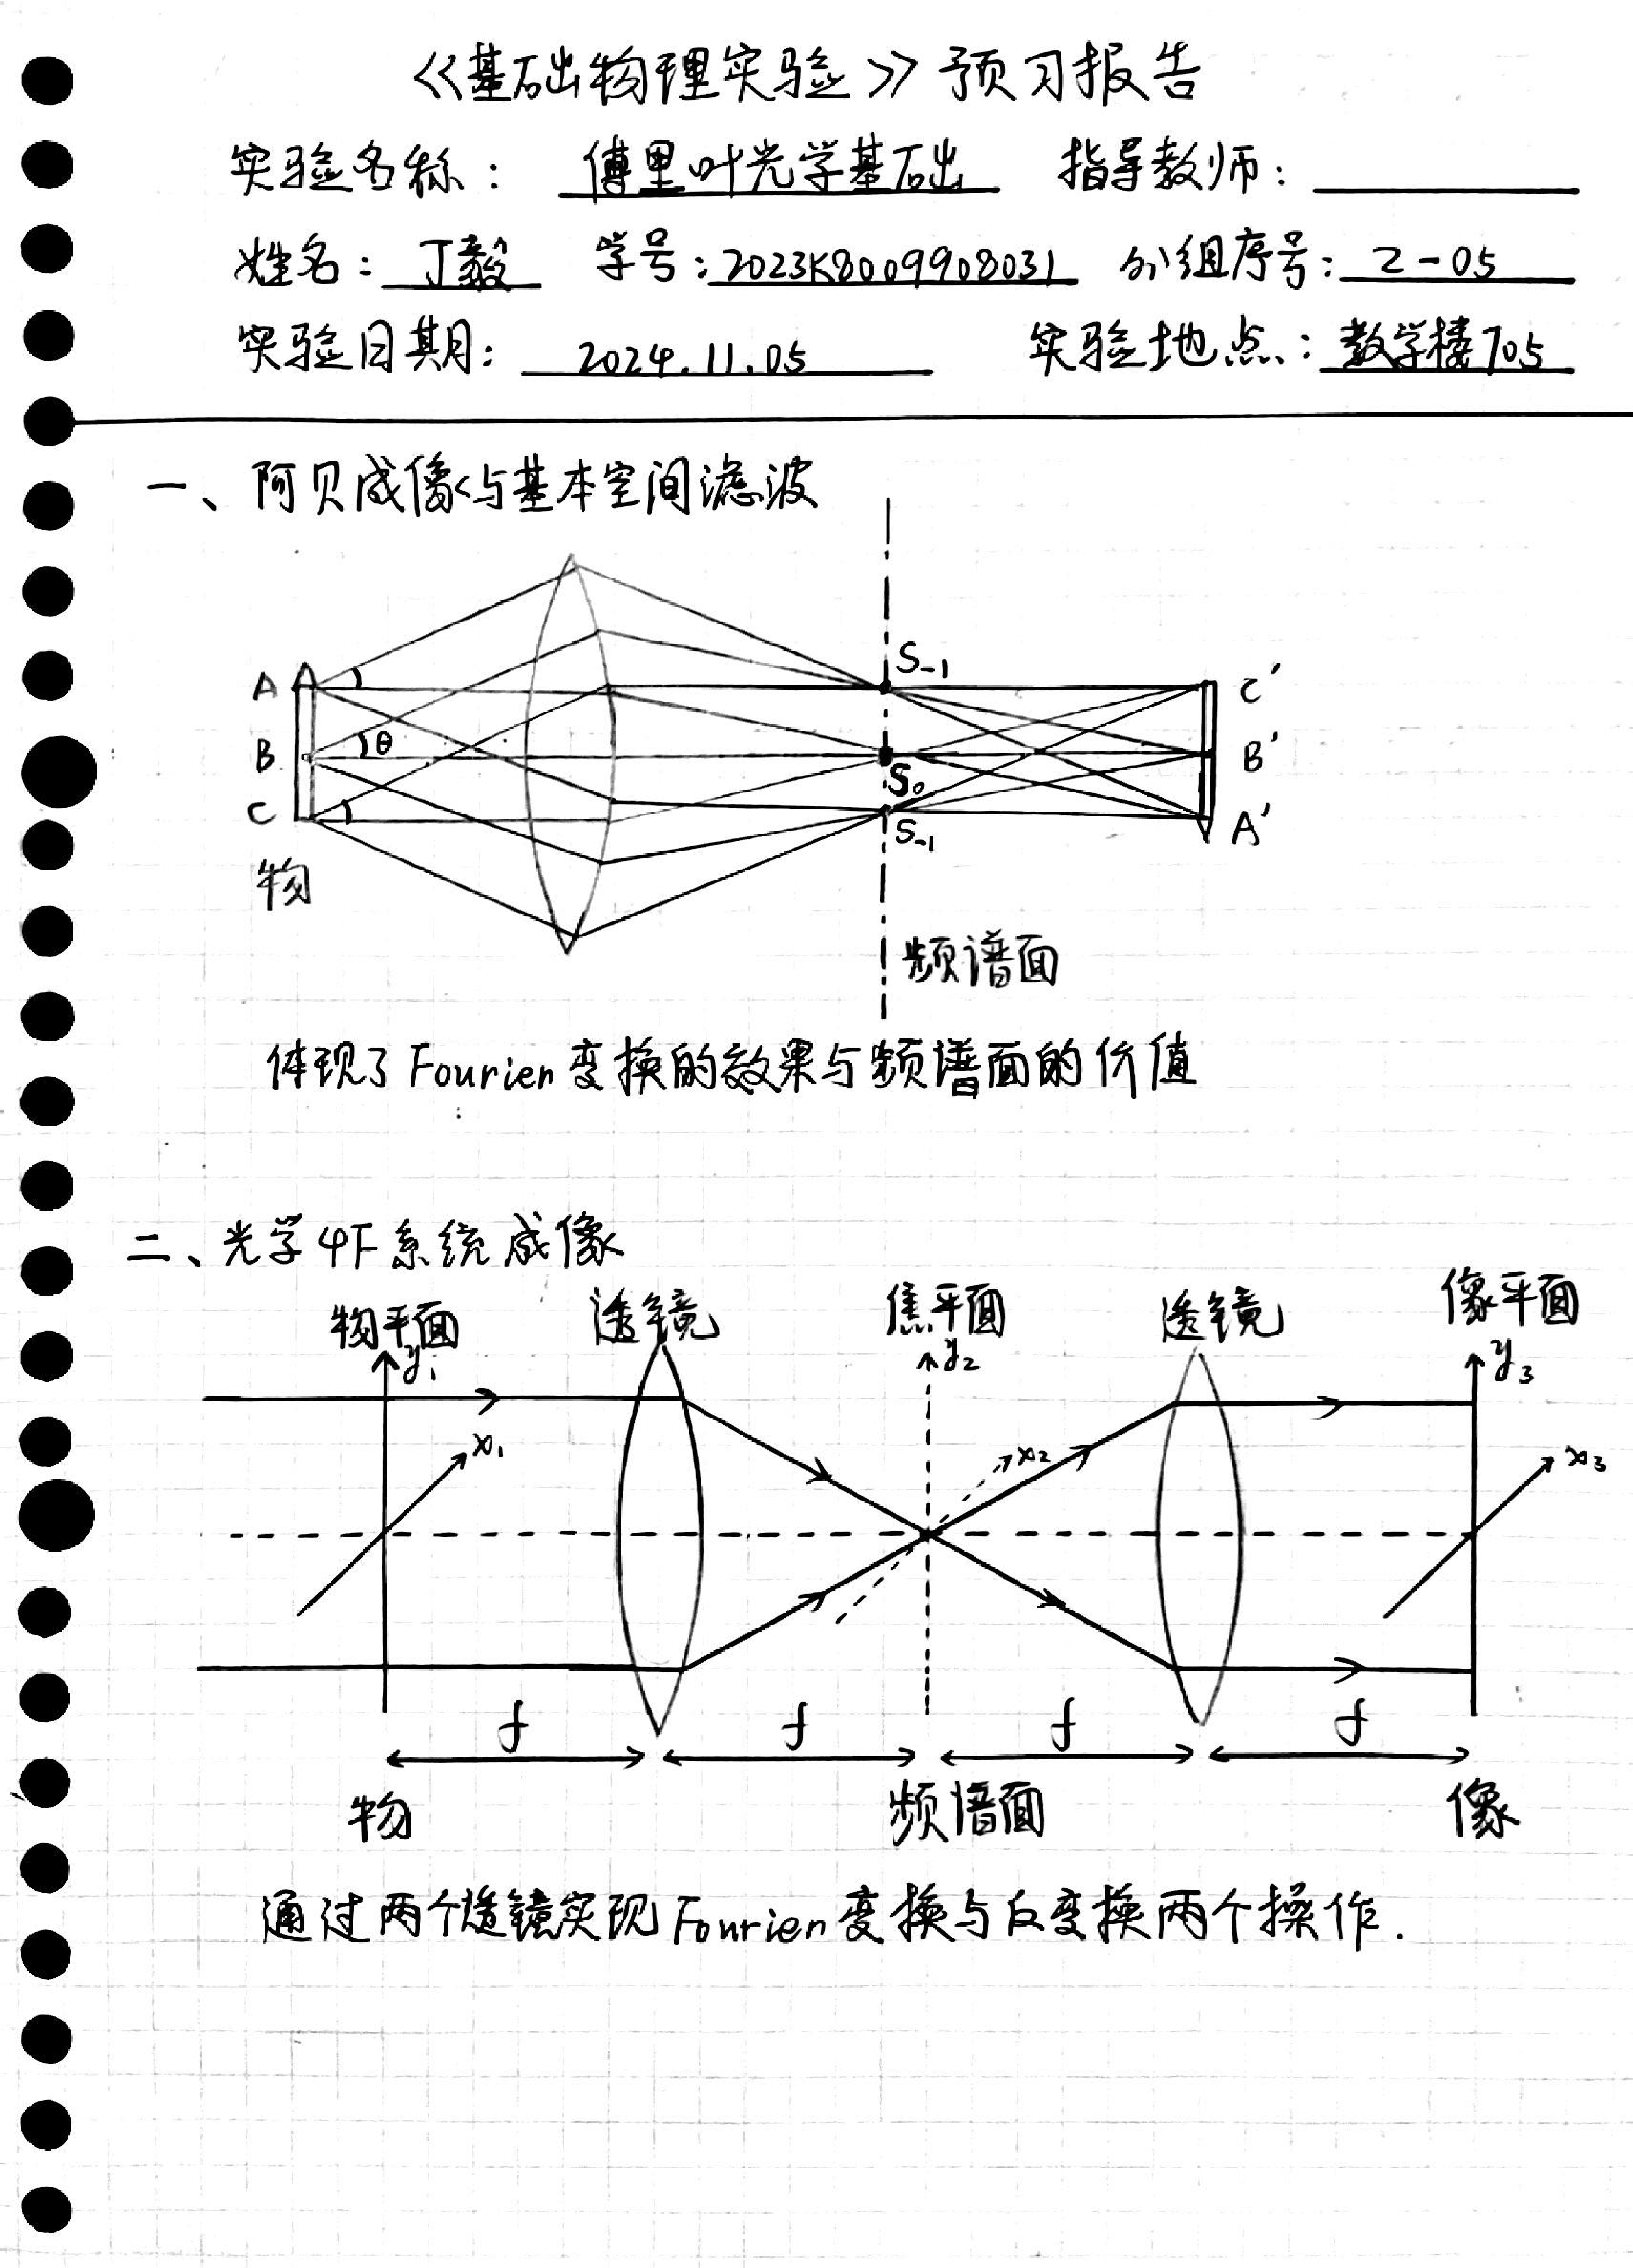
\includepdf[pages=1, width=480pt]{pdf/预习报告-2-05组-丁毅-傅里叶光学-2024.11.5-张秋琳.pdf}
\end{figure}
\includepdf[pages={2}]{pdf/预习报告-2-05组-丁毅-傅里叶光学-2024.11.5-张秋琳.pdf}

\section*{附录 B\hspace*{20pt} Matlab 源码}
\addcontentsline{toc}{section}{附录 B\hspace*{6pt} Matlab 源码} 
\thispagestyle{fancy} 
\lstinputlisting{d:/a_RemoteRepo/GH.MatlabCodes/本科课程代码/基础物理实验/Ex_10_mfile.m}



\end{document}

% VScode 常用快捷键:

% F2:                       变量重命名
% Ctrl + Enter:             行中换行
% Alt + up/down:            上下移行
% 鼠标中键 + 移动:           快速多光标
% Shift + Alt + up/down:    上下复制
% Ctrl + left/right:        左右跳单词
% Ctrl + Backspace/Delete:  左右删单词    
% Shift + Delete:           删除此行
% Ctrl + J:                 打开 VScode 下栏(输出栏)
% Ctrl + B:                 打开 VScode 左栏(目录栏)
% Ctrl + `:                 打开 VScode 终端栏
% Ctrl + 0:                 定位文件
% Ctrl + Tab:               切换已打开的文件(切标签)
% Ctrl + Shift + P:         打开全局命令(设置)

% Latex 常用快捷键:

% Ctrl + Alt + J:           由代码定位到PDF


